\documentclass[11pt,a4paper]{article}
\usepackage[T1]{fontenc}
\usepackage{lmodern}
\usepackage[margin=2.2cm]{geometry}
\usepackage{graphicx}
\usepackage{float}
\usepackage{caption}
\usepackage{subcaption}
\usepackage{longtable}
\usepackage[table]{xcolor}
\captionsetup{font=small,labelfont=bf}
\setlength{\parskip}{0.5em}
\setlength{\parindent}{0pt}
\usepackage[hidelinks,bookmarksnumbered]{hyperref}

\title{S\&P 500 market analysis}
\author{Data as of 2026-11-19}
\date{}
\begin{document}
\maketitle
\begin{abstract}
A concise view of the S\&P 500 over the last five years: company fundamentals from SEC EDGAR filings and prices and dividends from Yahoo Finance, for the current members outside the Financials and Real Estate sectors. For each measure, the sectors are compared, then every sector's best and worst companies, then the two best and two worst sectors in more detail; a final section puts P/E and value side by side to find companies that are both cheap and rewarding. The full history since 2006, used for back-testing, and the data checks are in the appendix. Companies that left the index are not included, so the results carry survivorship bias; all returns include reinvested dividends and all amounts are in US dollars.
\end{abstract}
\tableofcontents
\newpage
\section{Introduction}
\label{sec:introduction}
\begin{table}[H]
\centering
\small
\begin{tabular}{p{3.4cm}p{8.6cm}rl}
\hline
GICS sector & What it covers & Companies & Fund \\
\hline
Communication Services & Telecommunication carriers, media, entertainment and interactive online platforms. & 19 & XLC \\
Consumer Discretionary & Goods and services households buy by choice: cars, retail, hotels, restaurants, leisure. & 47 & XLY \\
Consumer Staples & Goods households need regardless of the economy: food, beverages, tobacco, household products. & 33 & XLP \\
Energy & Oil, gas and coal: exploration, production, refining, and energy equipment and services. & 21 & XLE \\
Health Care & Pharmaceuticals, biotechnology, medical equipment and health-care providers. & 60 & XLV \\
Industrials & Capital goods, aerospace and defence, transport, and commercial and professional services. & 83 & XLI \\
Information Technology & Software, IT services, hardware, semiconductors and electronic equipment. & 76 & XLK \\
Materials & Chemicals, construction materials, containers and packaging, metals and mining. & 24 & XLB \\
Utilities & Electric, gas and water utilities and independent power producers. & 31 & XLU \\
\hline
\end{tabular}
\end{table}
Companies are grouped by the Global Industry Classification Standard (GICS), which S\&P and MSCI use to classify listed companies by their principal business. The report uses the GICS sectors, the top level of the classification; Financials and Real Estate are left out because the balance-sheet rules of value investing do not fit banks, insurers and real-estate trusts. Each sector is compared with its SPDR sector fund, which tracks the S\&P 500 sector index and includes dividends, and with the S\&P 500 total-return index.

Plots name companies by their ticker; Appendix \ref{app:tickers} gives each company's full name, grouped by sector and sorted by ticker. In plots of companies, solid lines are the best and dashed lines the worst by the measure of the section, and each colour is one company. Rankings in the main text use the last five years, and only companies with prices for the whole five years are ranked.

\section{Fundamentals: revenue and net income}
\label{sec:fundamentals}
Revenue and net income are the values first reported in each company's annual report (10-K) to the SEC, in US dollars; later restatements are not used. Sector totals sum the companies of a sector per fiscal year; they move when the number of reporting companies changes, especially before 2009, and the fiscal year of the data date is left out because it is not complete. Companies are ranked by annualised revenue growth over the last 5 years, $g = (V_T / V_0)^{1/Y} - 1$, with $V_0$ and $V_T$ the first and last annual revenue and $Y$ the years between them; a sector by the median of its companies.

\begin{figure}[H]
\centering
\begin{subfigure}[t]{0.480\textwidth}
\centering
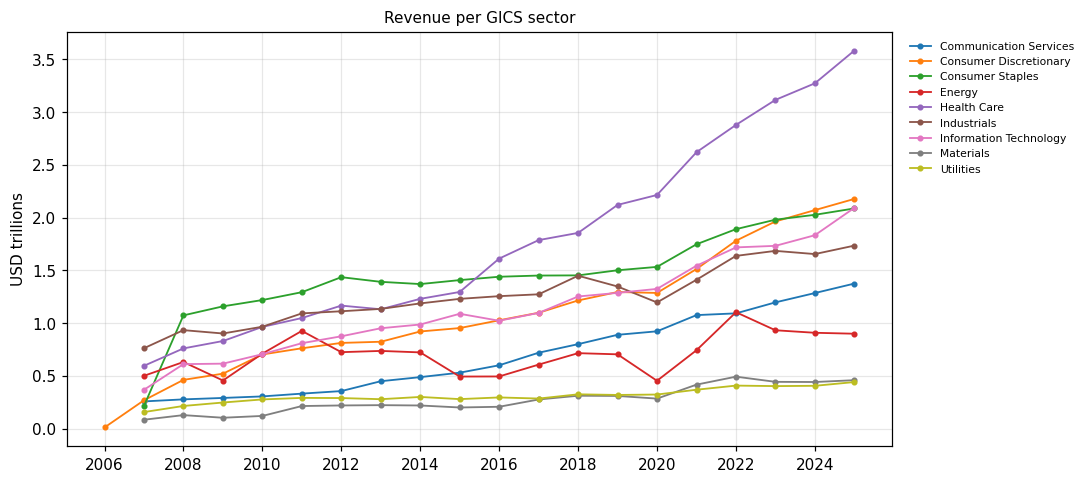
\includegraphics[width=\linewidth]{fundamentals/revenue.png}
\caption{Revenue}
\end{subfigure}\hfill
\begin{subfigure}[t]{0.480\textwidth}
\centering
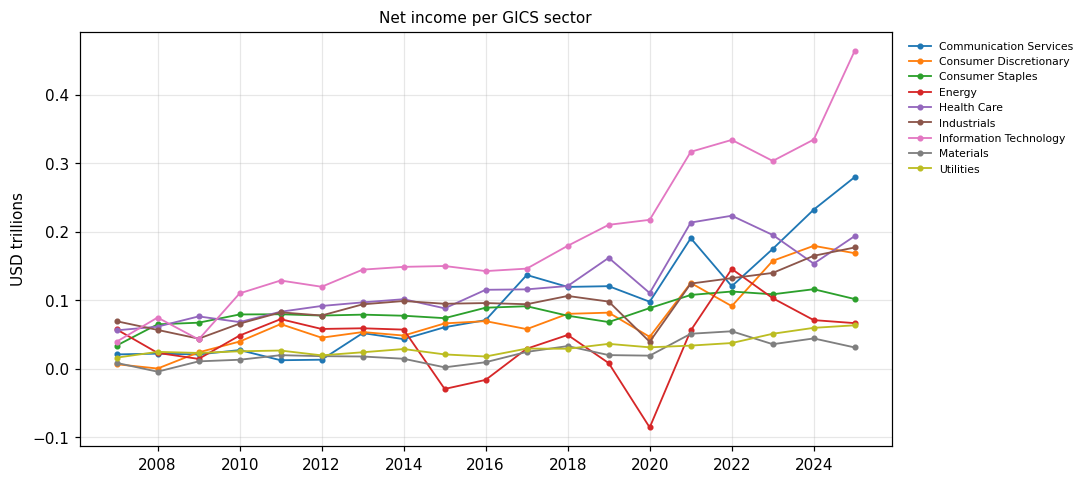
\includegraphics[width=\linewidth]{fundamentals/net_income.png}
\caption{Net income}
\end{subfigure}\hfill
\caption{Sum of first-reported annual (a) revenue and (b) net income over the companies of each GICS sector, USD trillions.}
\end{figure}
\begin{figure}[H]
\centering
\begin{subfigure}[t]{0.317\textwidth}
\centering
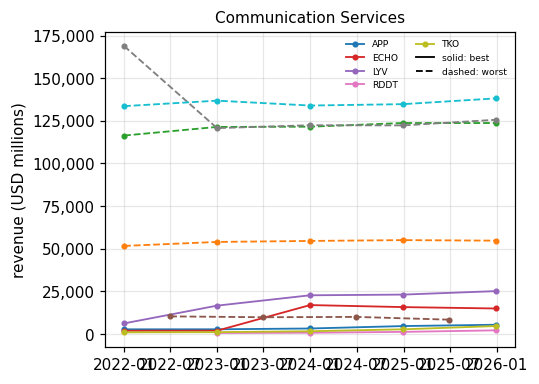
\includegraphics[width=\linewidth]{fundamentals/grid_communication_services.png}
\caption{Communication Services}
\end{subfigure}\hfill
\begin{subfigure}[t]{0.317\textwidth}
\centering
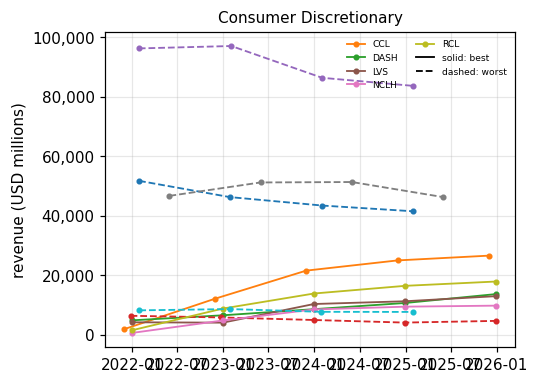
\includegraphics[width=\linewidth]{fundamentals/grid_consumer_discretionary.png}
\caption{Consumer Discretionary}
\end{subfigure}\hfill
\begin{subfigure}[t]{0.317\textwidth}
\centering
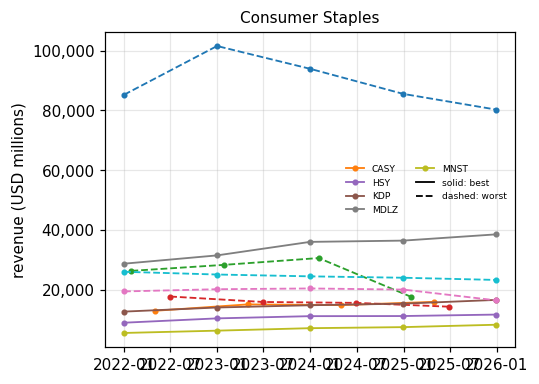
\includegraphics[width=\linewidth]{fundamentals/grid_consumer_staples.png}
\caption{Consumer Staples}
\end{subfigure}\hfill
\par\medskip
\begin{subfigure}[t]{0.317\textwidth}
\centering
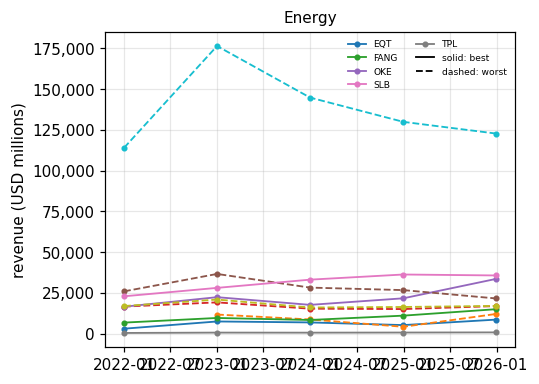
\includegraphics[width=\linewidth]{fundamentals/grid_energy.png}
\caption{Energy}
\end{subfigure}\hfill
\begin{subfigure}[t]{0.317\textwidth}
\centering
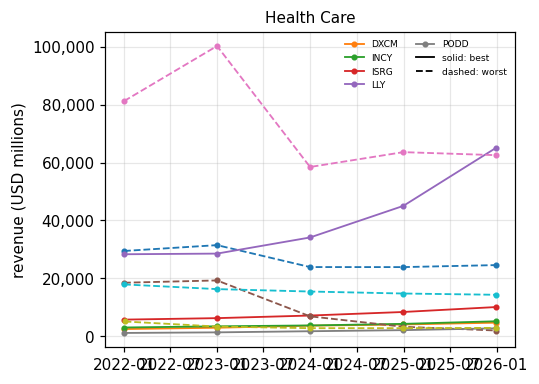
\includegraphics[width=\linewidth]{fundamentals/grid_health_care.png}
\caption{Health Care}
\end{subfigure}\hfill
\begin{subfigure}[t]{0.317\textwidth}
\centering
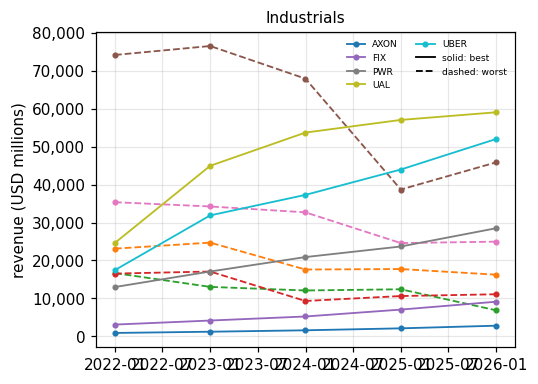
\includegraphics[width=\linewidth]{fundamentals/grid_industrials.png}
\caption{Industrials}
\end{subfigure}\hfill
\par\medskip
\begin{subfigure}[t]{0.317\textwidth}
\centering
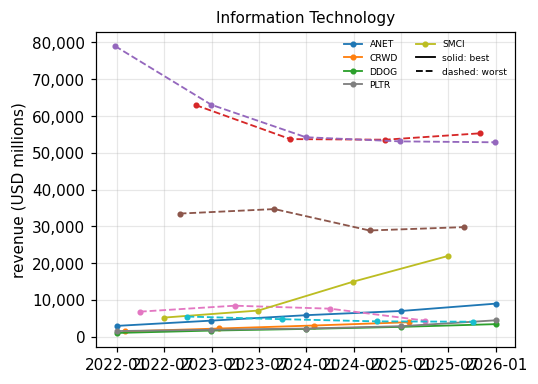
\includegraphics[width=\linewidth]{fundamentals/grid_information_technology.png}
\caption{Information Technology}
\end{subfigure}\hfill
\begin{subfigure}[t]{0.317\textwidth}
\centering
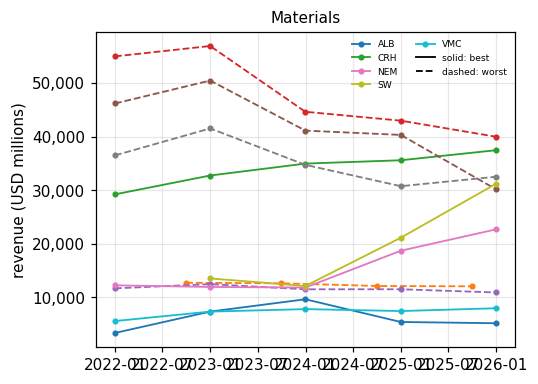
\includegraphics[width=\linewidth]{fundamentals/grid_materials.png}
\caption{Materials}
\end{subfigure}\hfill
\begin{subfigure}[t]{0.317\textwidth}
\centering
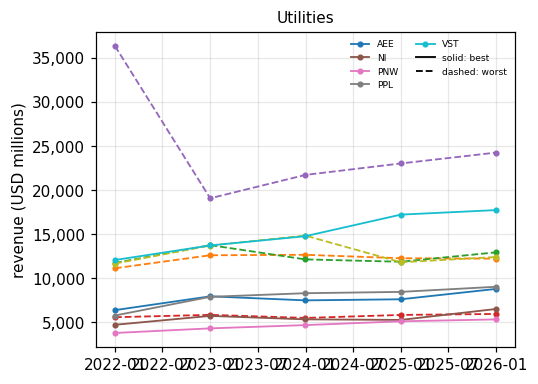
\includegraphics[width=\linewidth]{fundamentals/grid_utilities.png}
\caption{Utilities}
\end{subfigure}\hfill
\caption{Annual revenue, per GICS sector, of the 5 companies with the highest (solid) and lowest (dashed) revenue growth over the last 5 years; USD millions.}
\end{figure}
\subsection{Overview}
Over the last 5 years, Communication Services (11.1\% a year median growth) and Information Technology grew revenue fastest, Materials (2.3\% a year) and Health Care slowest. The full history of every sector is in Appendix \ref{app:fundamentals}.

\begin{figure}[H]
\centering
\begin{subfigure}[t]{0.480\textwidth}
\centering
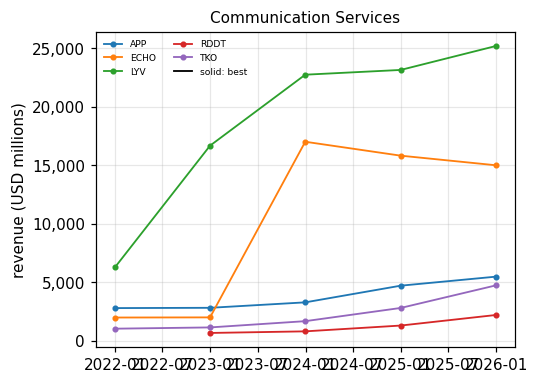
\includegraphics[width=\linewidth]{fundamentals/best_communication_services.png}
\caption{Communication Services}
\end{subfigure}\hfill
\begin{subfigure}[t]{0.480\textwidth}
\centering
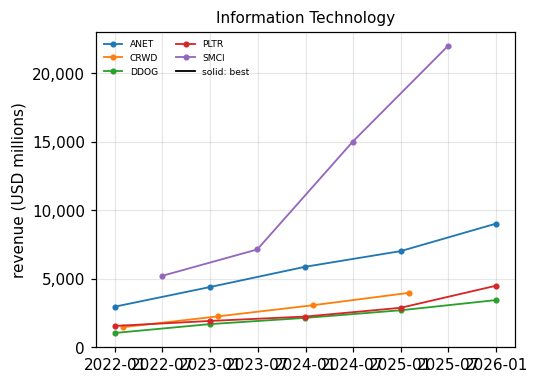
\includegraphics[width=\linewidth]{fundamentals/best_information_technology.png}
\caption{Information Technology}
\end{subfigure}\hfill
\caption{The two sectors with the highest median revenue growth over the last 5 years, (a) Communication Services and (b) Information Technology, with the revenue of their 5 fastest-growing companies; USD millions.}
\end{figure}
\begin{figure}[H]
\centering
\begin{subfigure}[t]{0.480\textwidth}
\centering
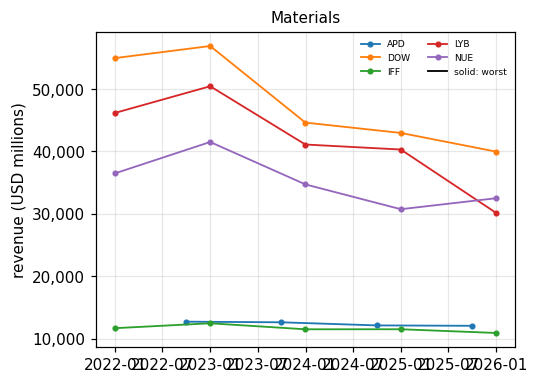
\includegraphics[width=\linewidth]{fundamentals/worst_materials.png}
\caption{Materials}
\end{subfigure}\hfill
\begin{subfigure}[t]{0.480\textwidth}
\centering
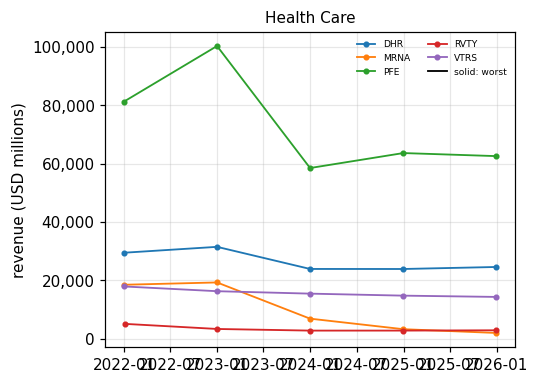
\includegraphics[width=\linewidth]{fundamentals/worst_health_care.png}
\caption{Health Care}
\end{subfigure}\hfill
\caption{The two sectors with the lowest median revenue growth, (a) Materials and (b) Health Care, with the revenue of their 5 slowest-growing companies; USD millions.}
\end{figure}
\section{Total return}
\label{sec:total_return}
Growth of one US dollar invested with dividends reinvested. Companies are ranked by annualised total return over the last 5 years, $r = (P_T / P_0)^{1/Y} - 1$, with $P$ the dividend-adjusted price; a sector by the return of its fund.

\begin{figure}[H]
\centering
\begin{subfigure}[t]{0.970\textwidth}
\centering
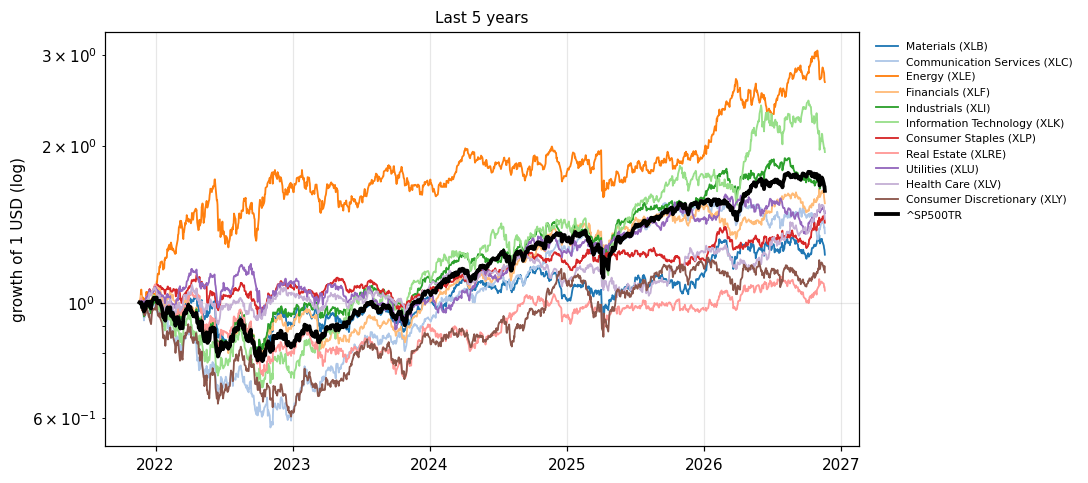
\includegraphics[width=\linewidth]{total_return/summary_recent.png}
\caption{Last 5 years}
\end{subfigure}\hfill
\par\medskip
\begin{subfigure}[t]{0.970\textwidth}
\centering
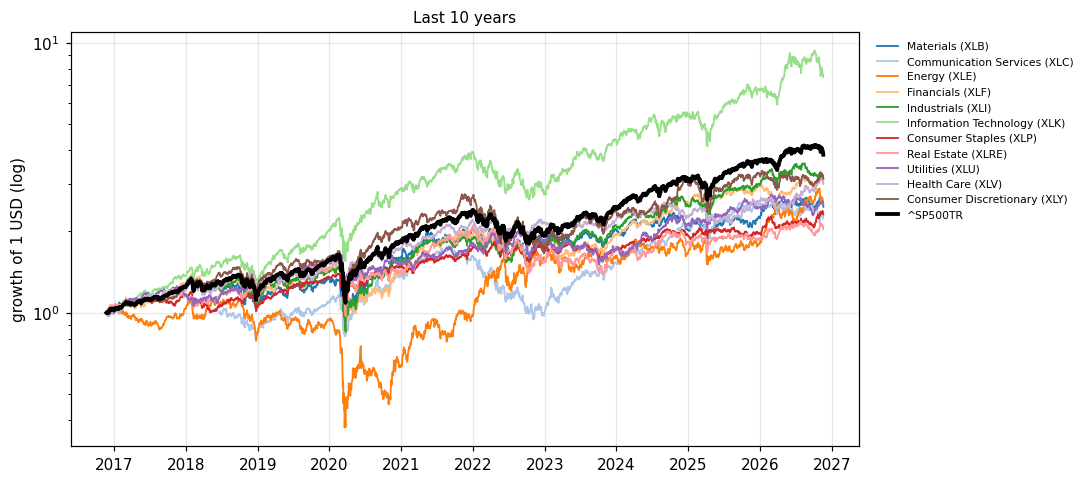
\includegraphics[width=\linewidth]{total_return/summary_long.png}
\caption{Last 10 years}
\end{subfigure}\hfill
\par\medskip
\begin{subfigure}[t]{0.970\textwidth}
\centering
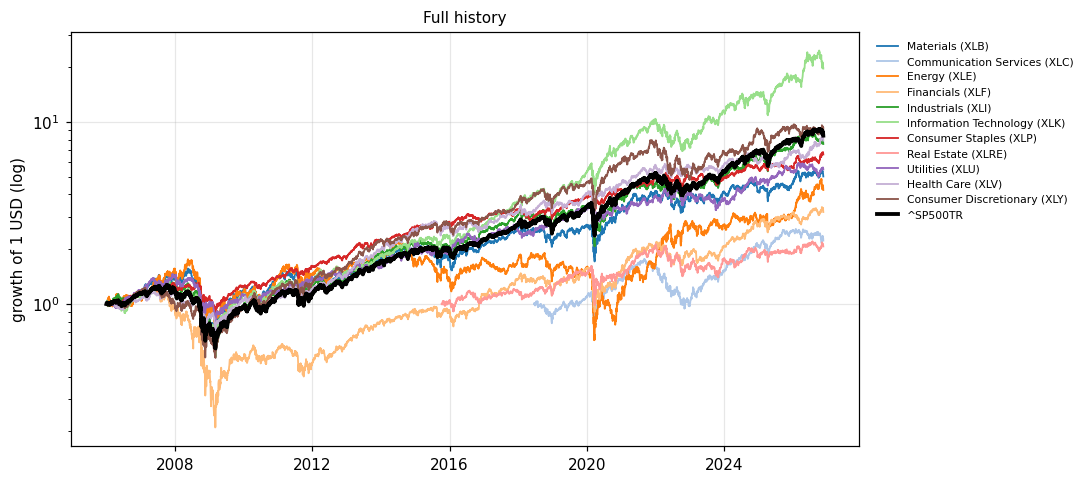
\includegraphics[width=\linewidth]{total_return/summary_full.png}
\caption{Full history}
\end{subfigure}\hfill
\caption{Growth of 1 USD with dividends reinvested for each GICS sector fund and the S\&P 500 (black), over (a) the last 5 years, (b) the last 10 years and (c) the full history since 2006; each view starts at 1, log scale.}
\end{figure}
\begin{figure}[H]
\centering
\begin{subfigure}[t]{0.317\textwidth}
\centering
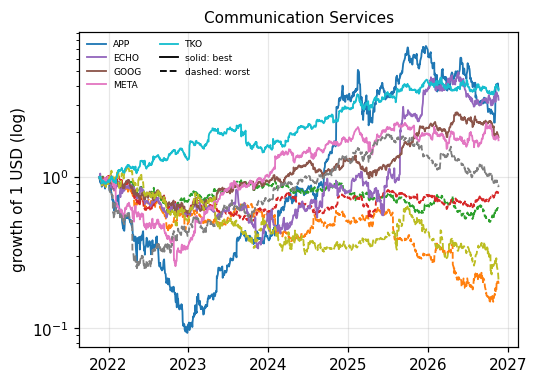
\includegraphics[width=\linewidth]{total_return/grid_communication_services.png}
\caption{Communication Services}
\end{subfigure}\hfill
\begin{subfigure}[t]{0.317\textwidth}
\centering
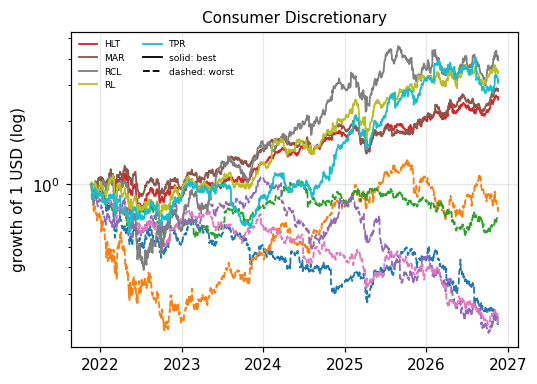
\includegraphics[width=\linewidth]{total_return/grid_consumer_discretionary.png}
\caption{Consumer Discretionary}
\end{subfigure}\hfill
\begin{subfigure}[t]{0.317\textwidth}
\centering
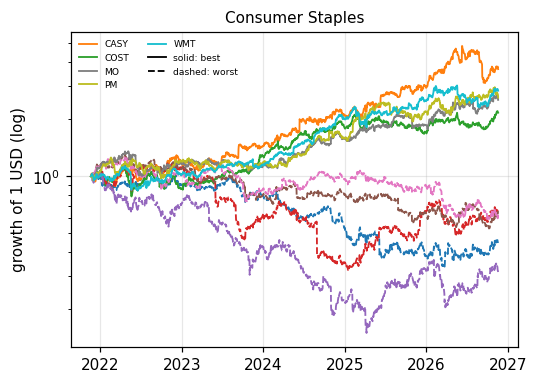
\includegraphics[width=\linewidth]{total_return/grid_consumer_staples.png}
\caption{Consumer Staples}
\end{subfigure}\hfill
\par\medskip
\begin{subfigure}[t]{0.317\textwidth}
\centering
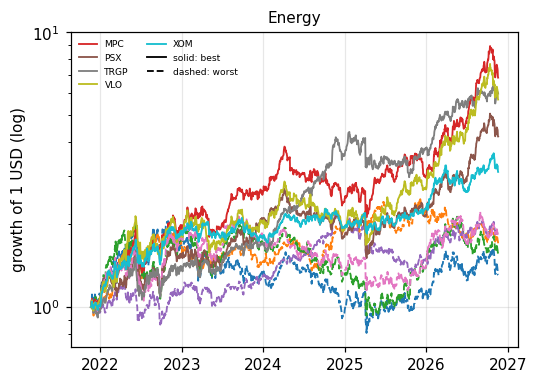
\includegraphics[width=\linewidth]{total_return/grid_energy.png}
\caption{Energy}
\end{subfigure}\hfill
\begin{subfigure}[t]{0.317\textwidth}
\centering
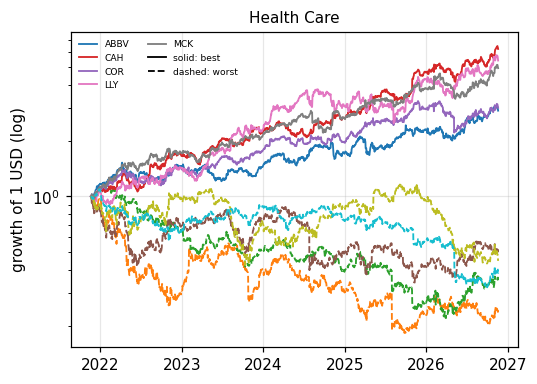
\includegraphics[width=\linewidth]{total_return/grid_health_care.png}
\caption{Health Care}
\end{subfigure}\hfill
\begin{subfigure}[t]{0.317\textwidth}
\centering
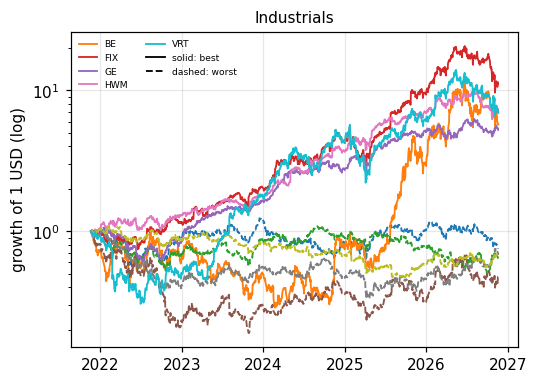
\includegraphics[width=\linewidth]{total_return/grid_industrials.png}
\caption{Industrials}
\end{subfigure}\hfill
\par\medskip
\begin{subfigure}[t]{0.317\textwidth}
\centering
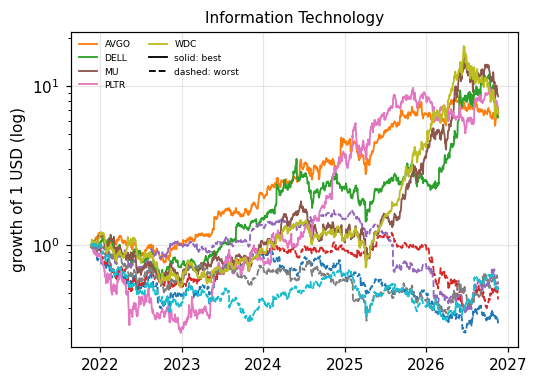
\includegraphics[width=\linewidth]{total_return/grid_information_technology.png}
\caption{Information Technology}
\end{subfigure}\hfill
\begin{subfigure}[t]{0.317\textwidth}
\centering
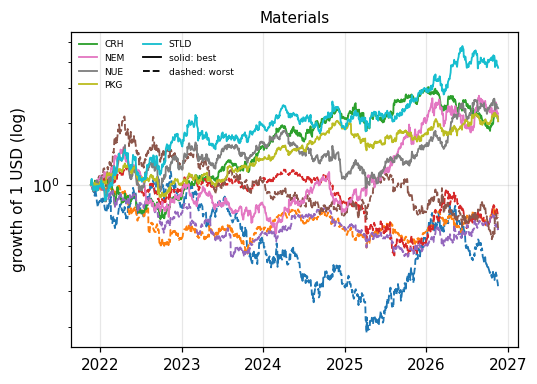
\includegraphics[width=\linewidth]{total_return/grid_materials.png}
\caption{Materials}
\end{subfigure}\hfill
\begin{subfigure}[t]{0.317\textwidth}
\centering
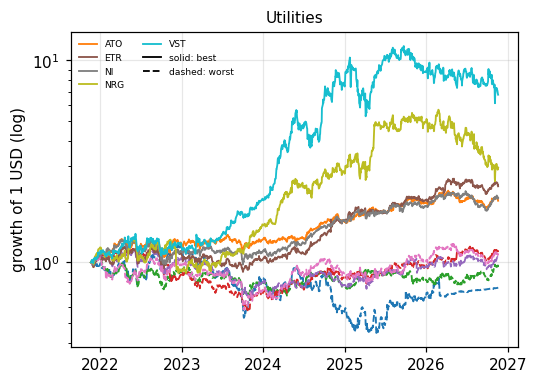
\includegraphics[width=\linewidth]{total_return/grid_utilities.png}
\caption{Utilities}
\end{subfigure}\hfill
\caption{Growth of 1 USD over the last 5 years, per GICS sector, for the 5 companies with the highest (solid) and lowest (dashed) total return; log scale.}
\end{figure}
\subsection{Overview}
Over the last 5 years the funds of Energy (21.6\% a year) and Information Technology returned the most, those of Consumer Discretionary (2.7\% a year) and Materials the least. The full history of every sector is in Appendix \ref{app:total_return}.

\begin{figure}[H]
\centering
\begin{subfigure}[t]{0.480\textwidth}
\centering
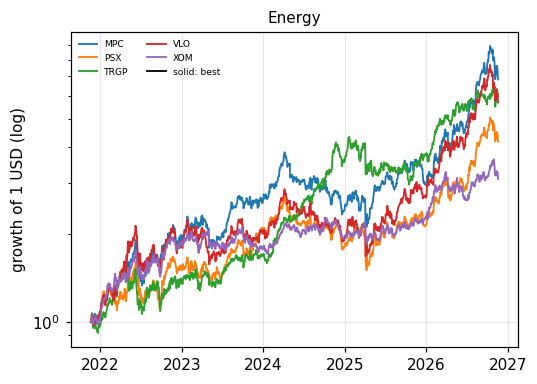
\includegraphics[width=\linewidth]{total_return/best_energy.png}
\caption{Energy}
\end{subfigure}\hfill
\begin{subfigure}[t]{0.480\textwidth}
\centering
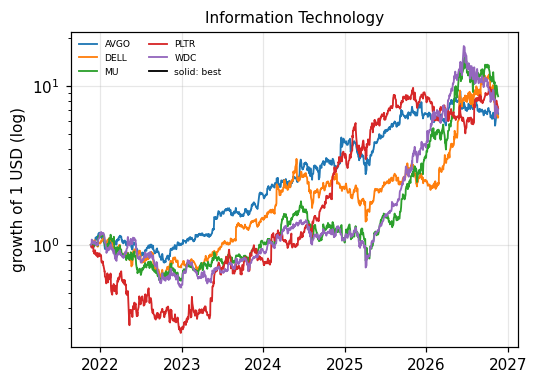
\includegraphics[width=\linewidth]{total_return/best_information_technology.png}
\caption{Information Technology}
\end{subfigure}\hfill
\caption{The two sectors whose funds returned the most over the last 5 years, (a) Energy and (b) Information Technology, with growth of 1 USD for their 5 best companies; log scale.}
\end{figure}
\begin{figure}[H]
\centering
\begin{subfigure}[t]{0.480\textwidth}
\centering
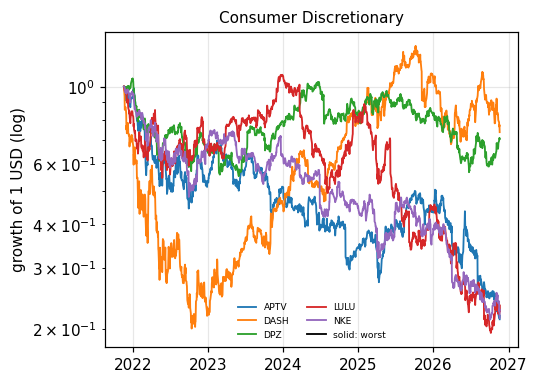
\includegraphics[width=\linewidth]{total_return/worst_consumer_discretionary.png}
\caption{Consumer Discretionary}
\end{subfigure}\hfill
\begin{subfigure}[t]{0.480\textwidth}
\centering
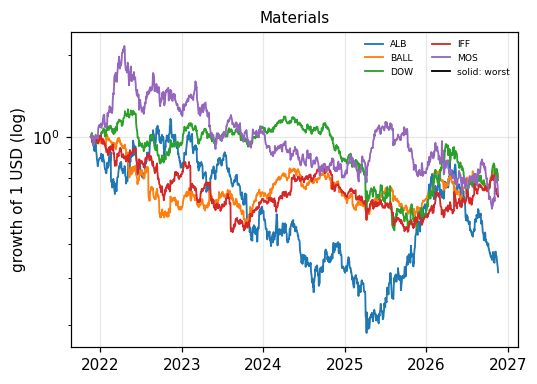
\includegraphics[width=\linewidth]{total_return/worst_materials.png}
\caption{Materials}
\end{subfigure}\hfill
\caption{The two sectors whose funds returned the least, (a) Consumer Discretionary and (b) Materials, with growth of 1 USD for their 5 worst companies; log scale.}
\end{figure}
\section{Relative return}
\label{sec:relative_return}
A series' growth divided by a benchmark's growth over the same period: above one it beat the benchmark. Sectors are compared with the S\&P 500 and companies with their sector fund, so a company's result is its performance within its sector. Ranking uses the annualised relative growth over the last 5 years.

\begin{figure}[H]
\centering
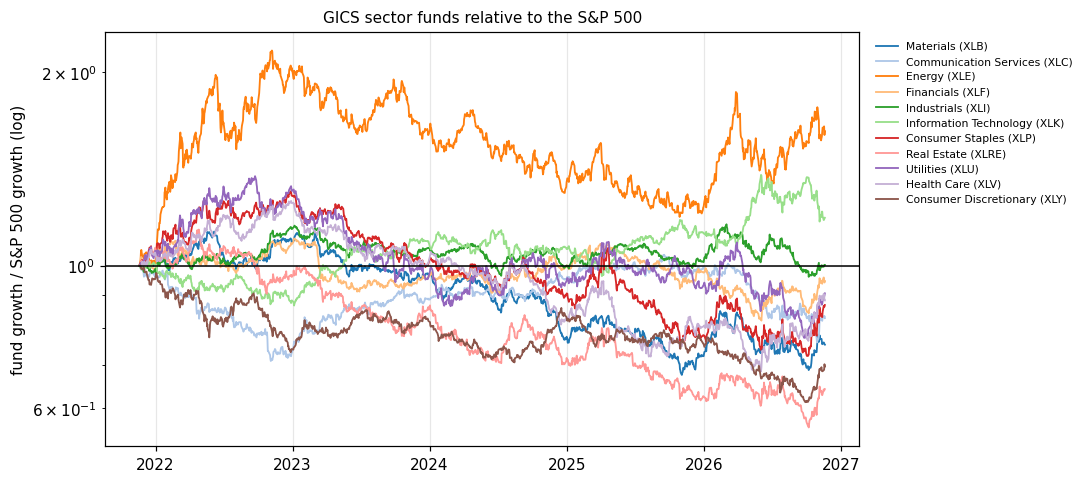
\includegraphics[width=1\textwidth]{relative_return/summary.png}
\caption{GICS sector funds relative to the S\&P 500 over the last 5 years, each starting at 1; above 1 the sector outperformed the market. Log scale.}
\end{figure}
\begin{figure}[H]
\centering
\begin{subfigure}[t]{0.317\textwidth}
\centering
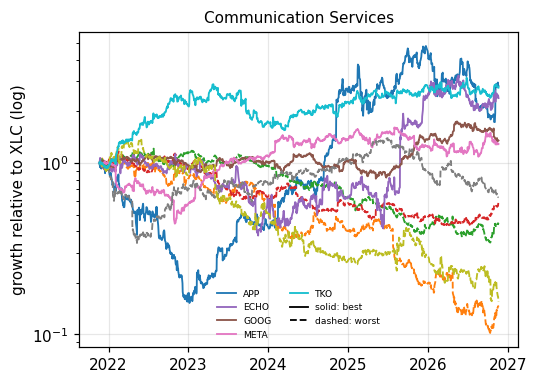
\includegraphics[width=\linewidth]{relative_return/grid_communication_services.png}
\caption{Communication Services}
\end{subfigure}\hfill
\begin{subfigure}[t]{0.317\textwidth}
\centering
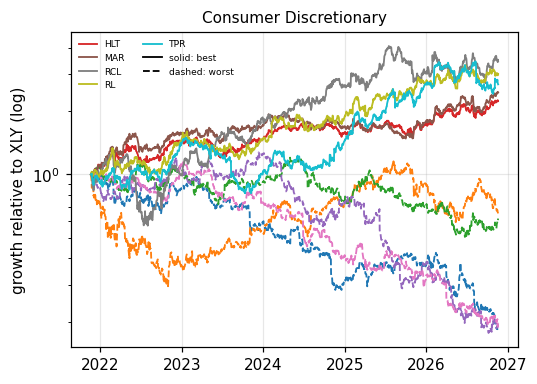
\includegraphics[width=\linewidth]{relative_return/grid_consumer_discretionary.png}
\caption{Consumer Discretionary}
\end{subfigure}\hfill
\begin{subfigure}[t]{0.317\textwidth}
\centering
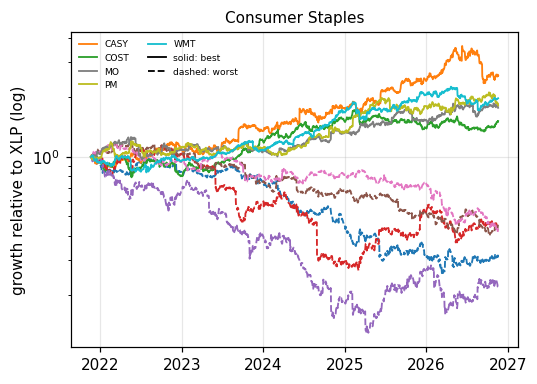
\includegraphics[width=\linewidth]{relative_return/grid_consumer_staples.png}
\caption{Consumer Staples}
\end{subfigure}\hfill
\par\medskip
\begin{subfigure}[t]{0.317\textwidth}
\centering
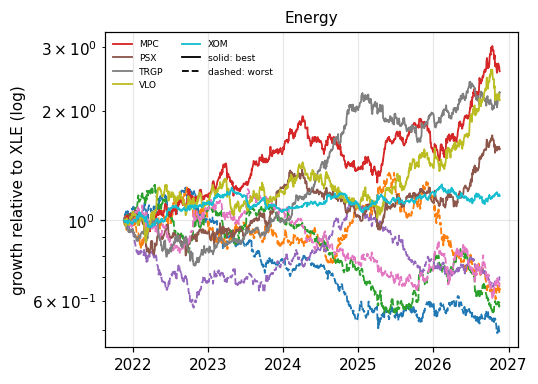
\includegraphics[width=\linewidth]{relative_return/grid_energy.png}
\caption{Energy}
\end{subfigure}\hfill
\begin{subfigure}[t]{0.317\textwidth}
\centering
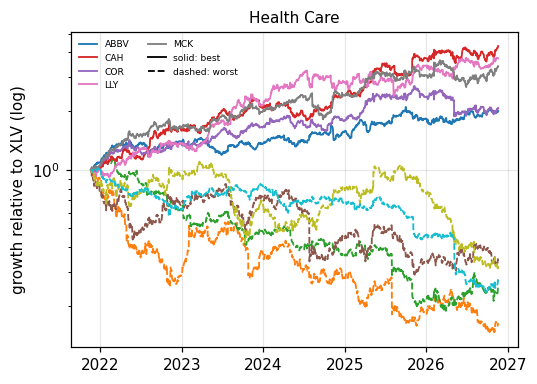
\includegraphics[width=\linewidth]{relative_return/grid_health_care.png}
\caption{Health Care}
\end{subfigure}\hfill
\begin{subfigure}[t]{0.317\textwidth}
\centering
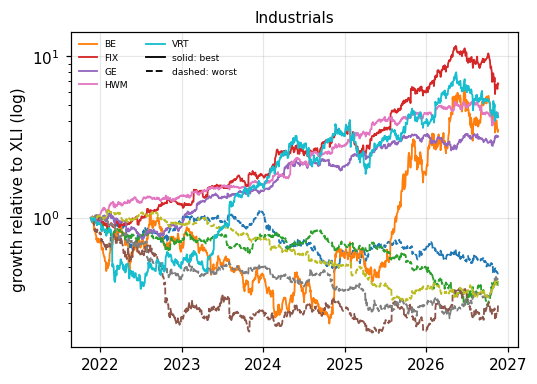
\includegraphics[width=\linewidth]{relative_return/grid_industrials.png}
\caption{Industrials}
\end{subfigure}\hfill
\par\medskip
\begin{subfigure}[t]{0.317\textwidth}
\centering
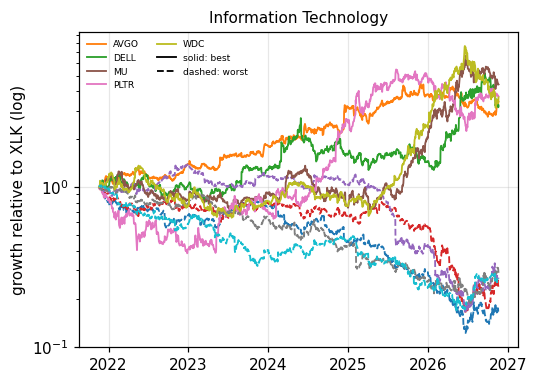
\includegraphics[width=\linewidth]{relative_return/grid_information_technology.png}
\caption{Information Technology}
\end{subfigure}\hfill
\begin{subfigure}[t]{0.317\textwidth}
\centering
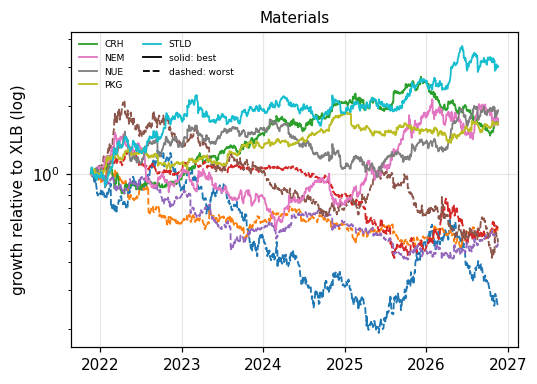
\includegraphics[width=\linewidth]{relative_return/grid_materials.png}
\caption{Materials}
\end{subfigure}\hfill
\begin{subfigure}[t]{0.317\textwidth}
\centering
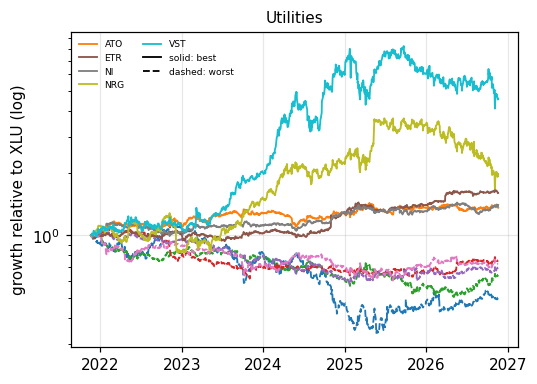
\includegraphics[width=\linewidth]{relative_return/grid_utilities.png}
\caption{Utilities}
\end{subfigure}\hfill
\caption{Growth relative to the sector fund over the last 5 years, per GICS sector, for the 5 companies that beat it most (solid) and trailed it most (dashed); log scale.}
\end{figure}
\subsection{Overview}
Against the S\&P 500, Energy (10.1\% a year) and Information Technology did best over the last 5 years, Consumer Discretionary (-7.0\% a year) and Materials worst. The full history of every sector is in Appendix \ref{app:relative_return}.

\begin{figure}[H]
\centering
\begin{subfigure}[t]{0.480\textwidth}
\centering
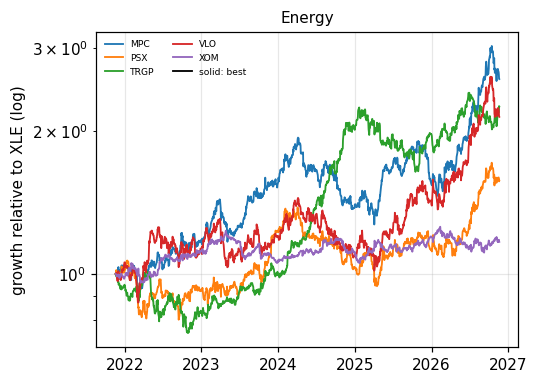
\includegraphics[width=\linewidth]{relative_return/best_energy.png}
\caption{Energy}
\end{subfigure}\hfill
\begin{subfigure}[t]{0.480\textwidth}
\centering
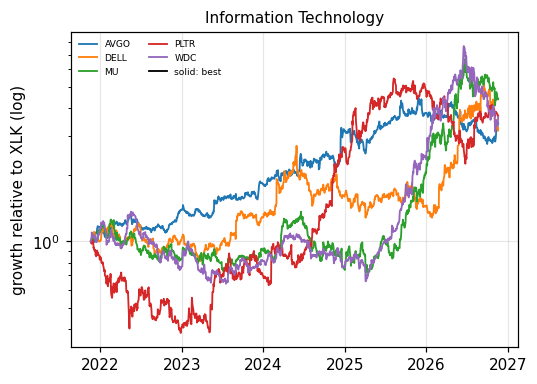
\includegraphics[width=\linewidth]{relative_return/best_information_technology.png}
\caption{Information Technology}
\end{subfigure}\hfill
\caption{The two sectors that beat the S\&P 500 most over the last 5 years, (a) Energy and (b) Information Technology, with their 5 companies that beat their sector fund most; growth relative to the fund, log scale.}
\end{figure}
\begin{figure}[H]
\centering
\begin{subfigure}[t]{0.480\textwidth}
\centering
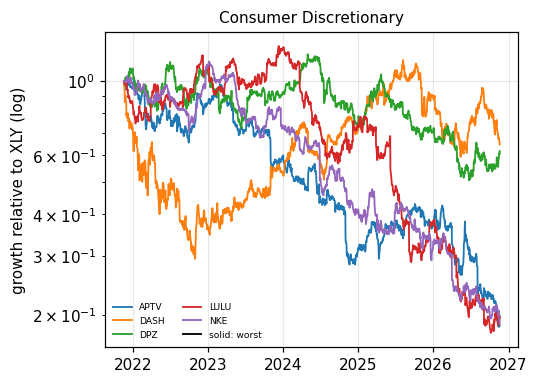
\includegraphics[width=\linewidth]{relative_return/worst_consumer_discretionary.png}
\caption{Consumer Discretionary}
\end{subfigure}\hfill
\begin{subfigure}[t]{0.480\textwidth}
\centering
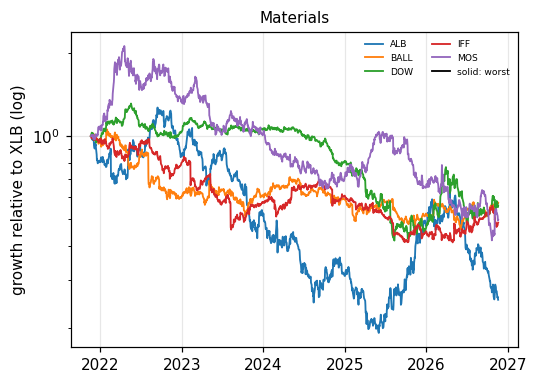
\includegraphics[width=\linewidth]{relative_return/worst_materials.png}
\caption{Materials}
\end{subfigure}\hfill
\caption{The two sectors that trailed the S\&P 500 most, (a) Consumer Discretionary and (b) Materials, with their 5 companies that trailed their sector fund most; growth relative to the fund, log scale.}
\end{figure}
\section{Price-to-earnings ratio}
\label{sec:pe}
The P/E divides the share price by the latest first-reported annual diluted earnings per share filed before the day, with earnings per share on the price's split basis; it changes in steps when a new annual report is filed, and companies with zero or negative earnings have none. A company is ranked by its median P/E over the last 5 years and a sector by the median of its companies; the lowest is best, as value investing looks for cheap earnings. The correlation of P/E and price changes is in Appendix \ref{app:pe}.

\begin{figure}[H]
\centering
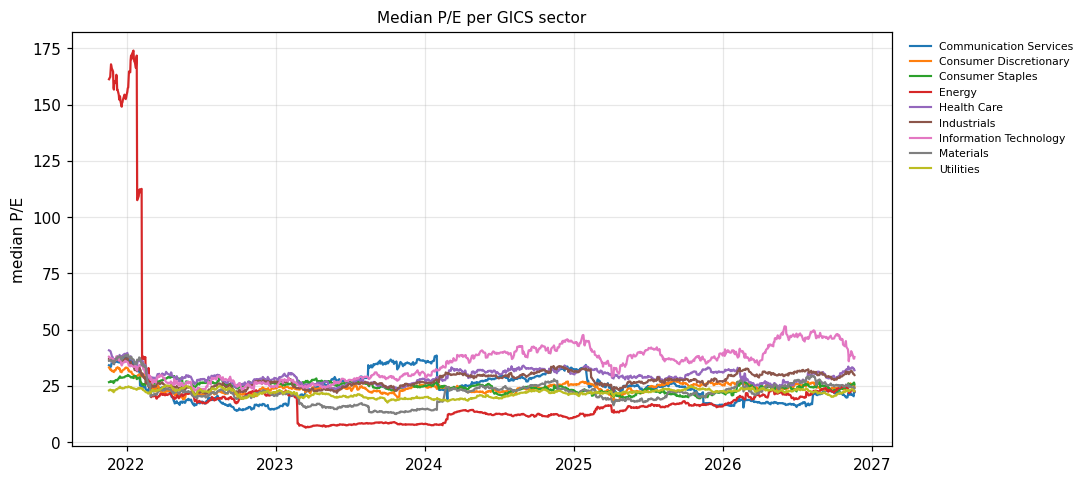
\includegraphics[width=1\textwidth]{pe/summary.png}
\caption{Median P/E of the companies in each GICS sector over the last 5 years.}
\end{figure}
\begin{figure}[H]
\centering
\begin{subfigure}[t]{0.317\textwidth}
\centering
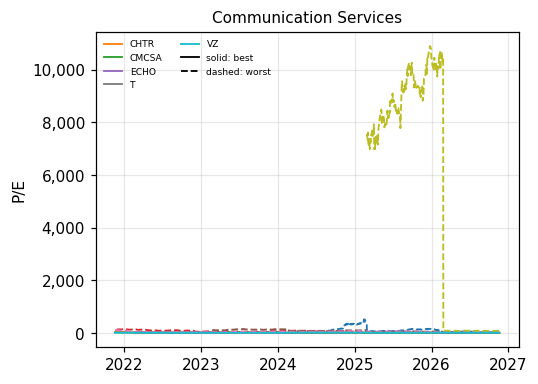
\includegraphics[width=\linewidth]{pe/grid_communication_services.png}
\caption{Communication Services}
\end{subfigure}\hfill
\begin{subfigure}[t]{0.317\textwidth}
\centering
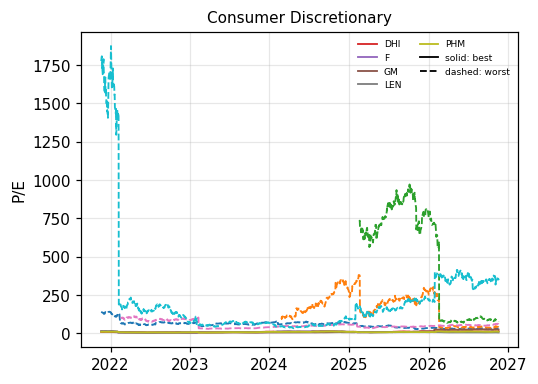
\includegraphics[width=\linewidth]{pe/grid_consumer_discretionary.png}
\caption{Consumer Discretionary}
\end{subfigure}\hfill
\begin{subfigure}[t]{0.317\textwidth}
\centering
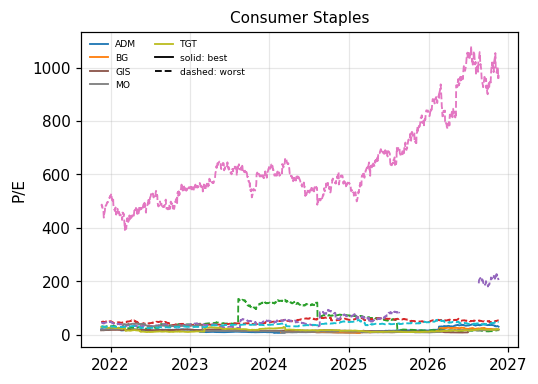
\includegraphics[width=\linewidth]{pe/grid_consumer_staples.png}
\caption{Consumer Staples}
\end{subfigure}\hfill
\par\medskip
\begin{subfigure}[t]{0.317\textwidth}
\centering
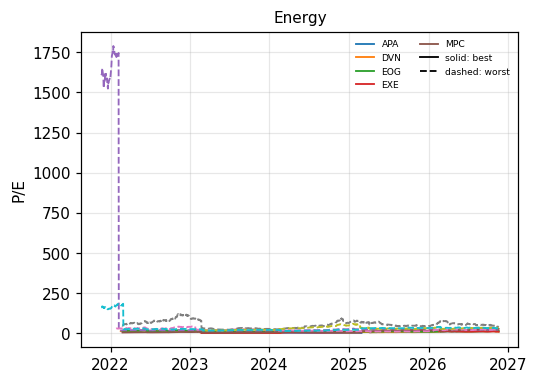
\includegraphics[width=\linewidth]{pe/grid_energy.png}
\caption{Energy}
\end{subfigure}\hfill
\begin{subfigure}[t]{0.317\textwidth}
\centering
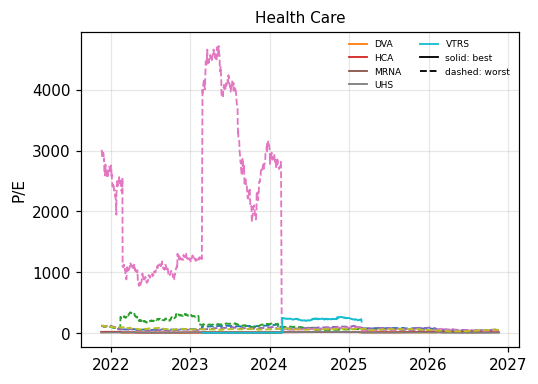
\includegraphics[width=\linewidth]{pe/grid_health_care.png}
\caption{Health Care}
\end{subfigure}\hfill
\begin{subfigure}[t]{0.317\textwidth}
\centering
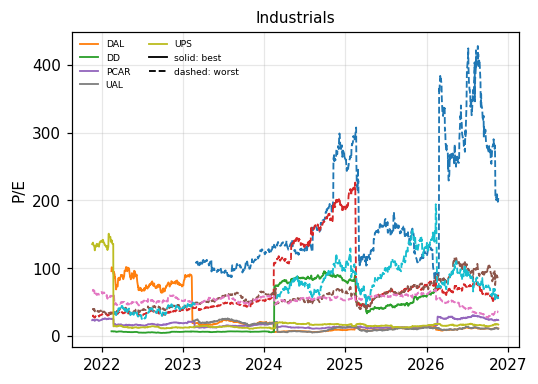
\includegraphics[width=\linewidth]{pe/grid_industrials.png}
\caption{Industrials}
\end{subfigure}\hfill
\par\medskip
\begin{subfigure}[t]{0.317\textwidth}
\centering
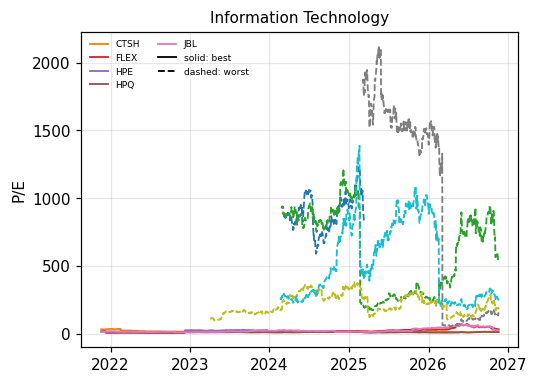
\includegraphics[width=\linewidth]{pe/grid_information_technology.png}
\caption{Information Technology}
\end{subfigure}\hfill
\begin{subfigure}[t]{0.317\textwidth}
\centering
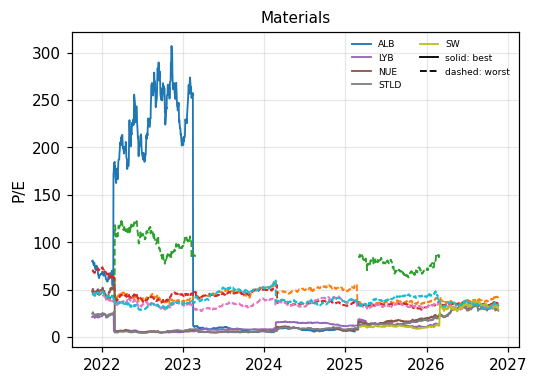
\includegraphics[width=\linewidth]{pe/grid_materials.png}
\caption{Materials}
\end{subfigure}\hfill
\begin{subfigure}[t]{0.317\textwidth}
\centering
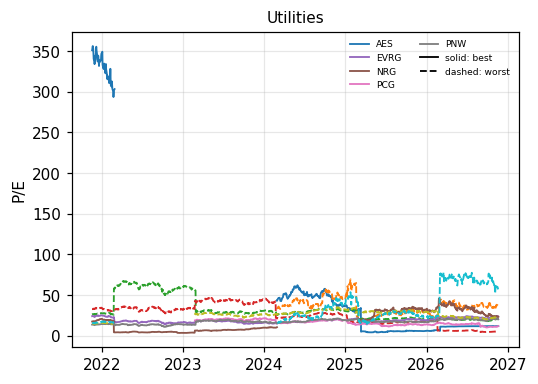
\includegraphics[width=\linewidth]{pe/grid_utilities.png}
\caption{Utilities}
\end{subfigure}\hfill
\caption{P/E over the last 5 years, per GICS sector, of the 5 companies with the lowest (solid) and highest (dashed) median P/E.}
\end{figure}
\subsection{Overview}
Over the last 5 years Energy (16.0) and Materials had the lowest median P/E, Information Technology (32.4) and Communication Services the highest. The full history of every sector is in Appendix \ref{app:pe}.

\begin{figure}[H]
\centering
\begin{subfigure}[t]{0.480\textwidth}
\centering
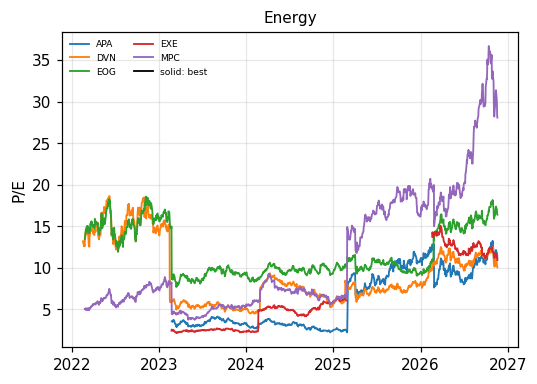
\includegraphics[width=\linewidth]{pe/best_energy.png}
\caption{Energy}
\end{subfigure}\hfill
\begin{subfigure}[t]{0.480\textwidth}
\centering
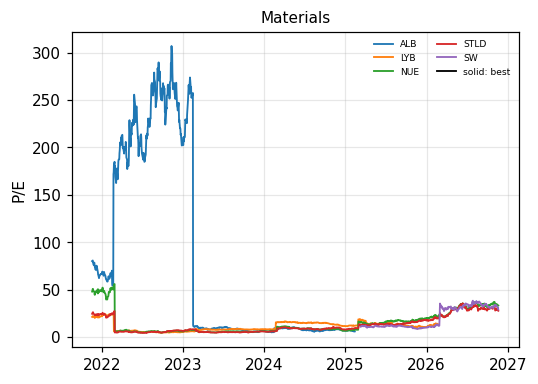
\includegraphics[width=\linewidth]{pe/best_materials.png}
\caption{Materials}
\end{subfigure}\hfill
\caption{The two sectors with the lowest median P/E over the last 5 years, (a) Energy and (b) Materials, with the P/E of their 5 cheapest companies.}
\end{figure}
\begin{figure}[H]
\centering
\begin{subfigure}[t]{0.480\textwidth}
\centering
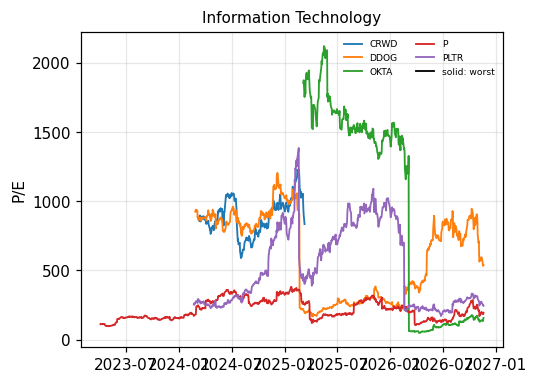
\includegraphics[width=\linewidth]{pe/worst_information_technology.png}
\caption{Information Technology}
\end{subfigure}\hfill
\begin{subfigure}[t]{0.480\textwidth}
\centering
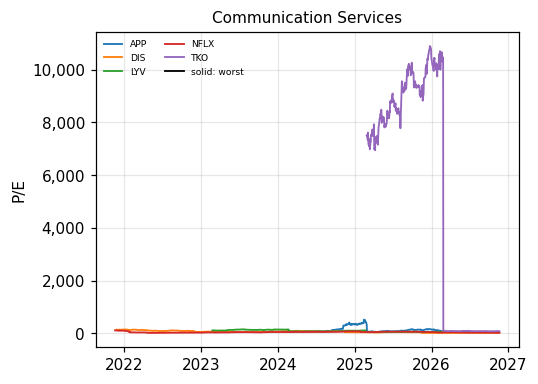
\includegraphics[width=\linewidth]{pe/worst_communication_services.png}
\caption{Communication Services}
\end{subfigure}\hfill
\caption{The two sectors with the highest median P/E, (a) Information Technology and (b) Communication Services, with the P/E of their 5 most expensive companies.}
\end{figure}
\section{P/E and value}
\label{sec:pe_value}
Value investing looks for companies that are cheap on earnings and still reward their holders. Across all companies, those with the lowest median P/E over the last 5 years are set beside those with the highest total return over the same years, and likewise for the highest P/E and the lowest return; every plot shows both measures for each company. Companies in both best lists: none. Companies in both worst lists: none. Finding such overlap is what the models aim for.

\begin{figure}[H]
\centering
\begin{subfigure}[t]{0.480\textwidth}
\centering
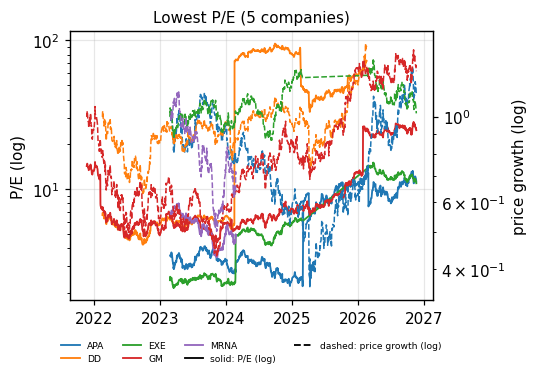
\includegraphics[width=\linewidth]{pe_value/low_pe.png}
\caption{Lowest P/E (5 companies)}
\end{subfigure}\hfill
\begin{subfigure}[t]{0.480\textwidth}
\centering
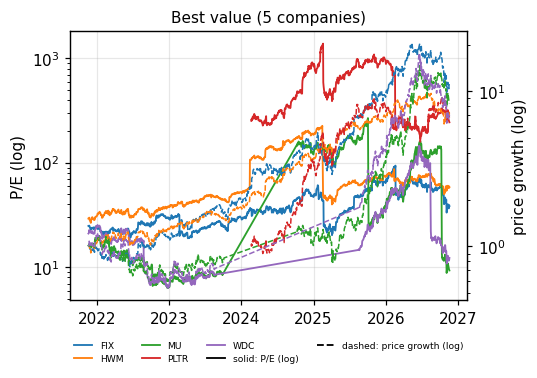
\includegraphics[width=\linewidth]{pe_value/best_value.png}
\caption{Best value (5 companies)}
\end{subfigure}\hfill
\caption{(a) The 5 companies with the lowest median P/E over the last 5 years (APA, EXE, MRNA, GM, DD) and (b) the 5 with the highest total return (FIX, MU, HWM, PLTR, WDC); for each company its P/E (solid, left axis) and price growth since the start of the window (dashed, right axis), log scales.}
\end{figure}
\begin{figure}[H]
\centering
\begin{subfigure}[t]{0.480\textwidth}
\centering
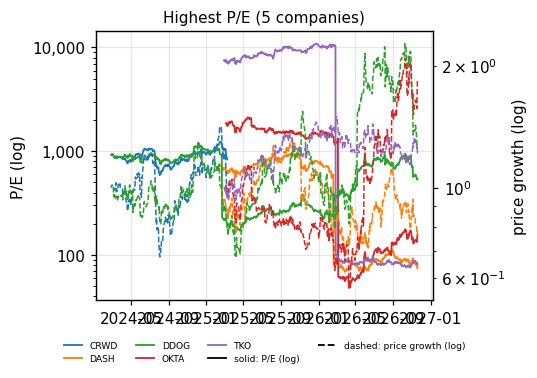
\includegraphics[width=\linewidth]{pe_value/high_pe.png}
\caption{Highest P/E (5 companies)}
\end{subfigure}\hfill
\begin{subfigure}[t]{0.480\textwidth}
\centering
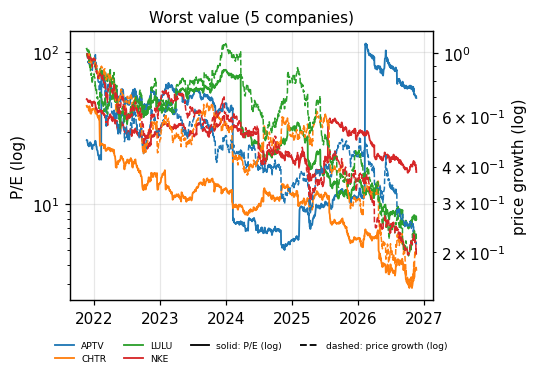
\includegraphics[width=\linewidth]{pe_value/worst_value.png}
\caption{Worst value (5 companies)}
\end{subfigure}\hfill
\caption{(a) The 5 companies with the highest median P/E over the last 5 years (TKO, OKTA, CRWD, DDOG, DASH) and (b) the 5 with the lowest total return (CHTR, SKYD, APTV, NKE, LULU); P/E (solid, left axis) and price growth (dashed, right axis), log scales.}
\end{figure}
\section{Dividend yield}
\label{sec:dividend_yield}
The trailing dividend yield is the sum of a company's dividends with an ex-date in the past twelve months divided by its share price, both on the same split basis, in percent; a company that paid no dividend in the window yields zero. A company is ranked by its mean yield over the last 5 years and a sector by the median of its companies; the highest is best.

\begin{figure}[H]
\centering
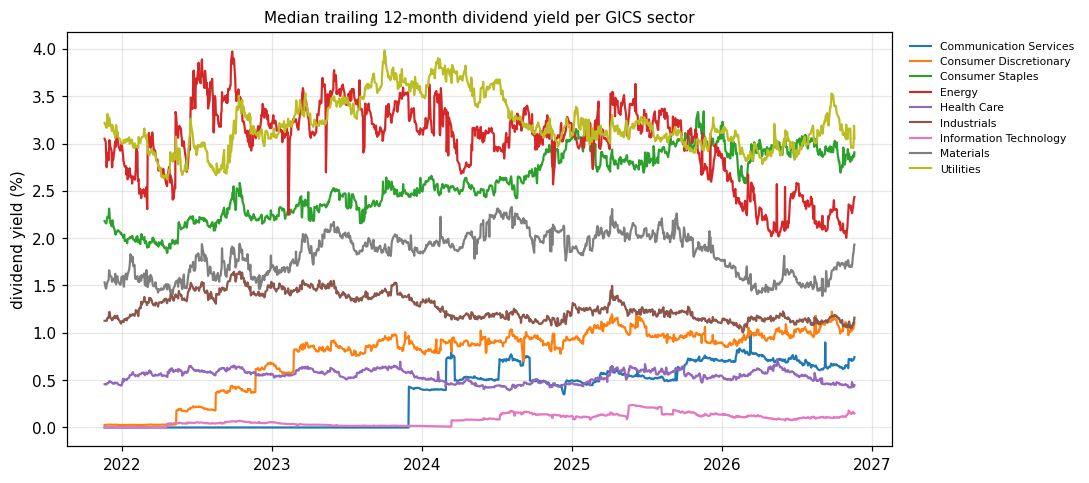
\includegraphics[width=1\textwidth]{dividend_yield/summary.png}
\caption{Median trailing 12-month dividend yield of the companies in each GICS sector over the last 5 years, percent.}
\end{figure}
\begin{figure}[H]
\centering
\begin{subfigure}[t]{0.317\textwidth}
\centering
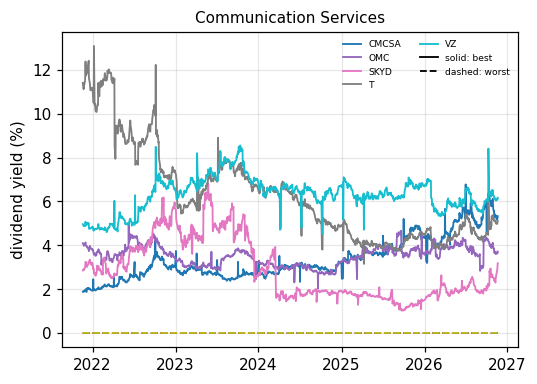
\includegraphics[width=\linewidth]{dividend_yield/grid_communication_services.png}
\caption{Communication Services}
\end{subfigure}\hfill
\begin{subfigure}[t]{0.317\textwidth}
\centering
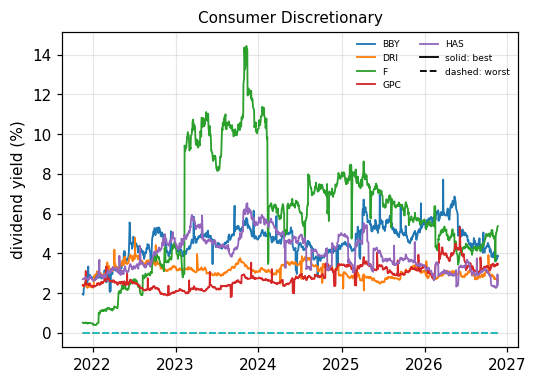
\includegraphics[width=\linewidth]{dividend_yield/grid_consumer_discretionary.png}
\caption{Consumer Discretionary}
\end{subfigure}\hfill
\begin{subfigure}[t]{0.317\textwidth}
\centering
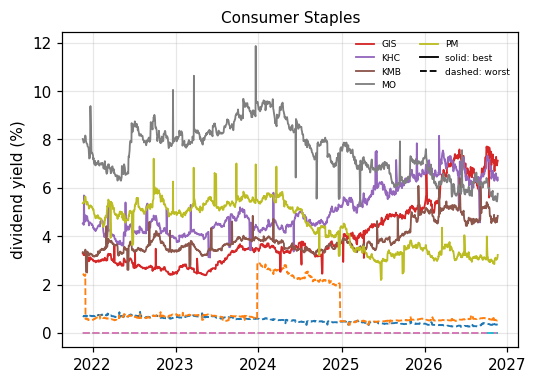
\includegraphics[width=\linewidth]{dividend_yield/grid_consumer_staples.png}
\caption{Consumer Staples}
\end{subfigure}\hfill
\par\medskip
\begin{subfigure}[t]{0.317\textwidth}
\centering
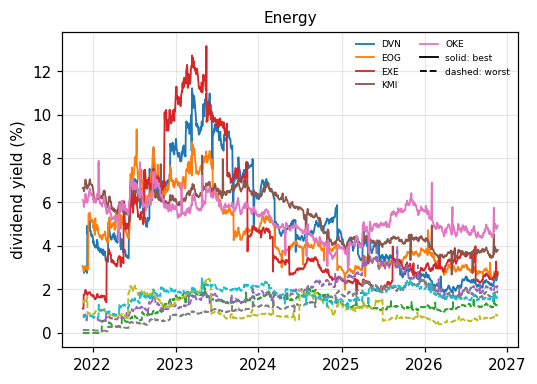
\includegraphics[width=\linewidth]{dividend_yield/grid_energy.png}
\caption{Energy}
\end{subfigure}\hfill
\begin{subfigure}[t]{0.317\textwidth}
\centering
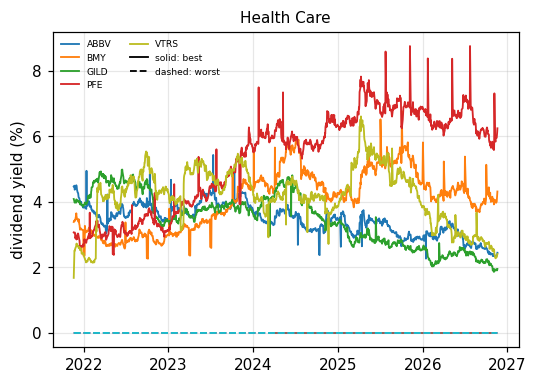
\includegraphics[width=\linewidth]{dividend_yield/grid_health_care.png}
\caption{Health Care}
\end{subfigure}\hfill
\begin{subfigure}[t]{0.317\textwidth}
\centering
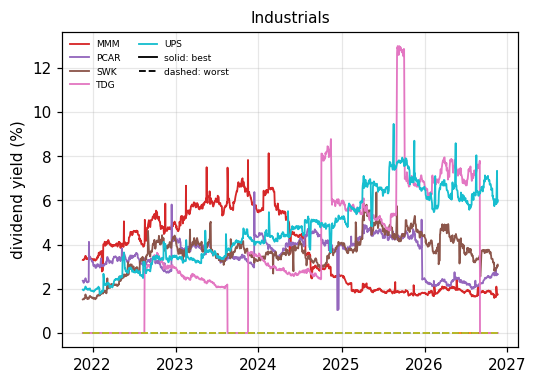
\includegraphics[width=\linewidth]{dividend_yield/grid_industrials.png}
\caption{Industrials}
\end{subfigure}\hfill
\par\medskip
\begin{subfigure}[t]{0.317\textwidth}
\centering
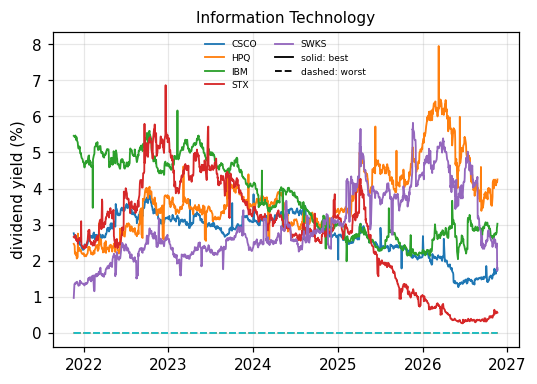
\includegraphics[width=\linewidth]{dividend_yield/grid_information_technology.png}
\caption{Information Technology}
\end{subfigure}\hfill
\begin{subfigure}[t]{0.317\textwidth}
\centering
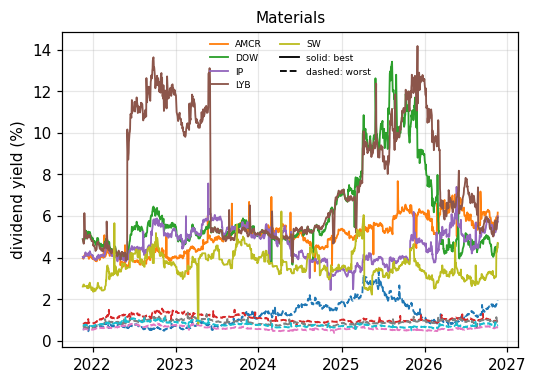
\includegraphics[width=\linewidth]{dividend_yield/grid_materials.png}
\caption{Materials}
\end{subfigure}\hfill
\begin{subfigure}[t]{0.317\textwidth}
\centering
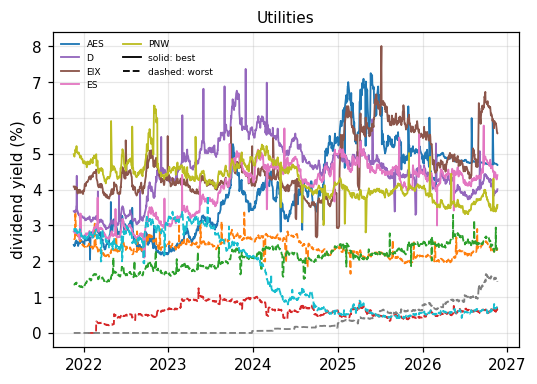
\includegraphics[width=\linewidth]{dividend_yield/grid_utilities.png}
\caption{Utilities}
\end{subfigure}\hfill
\caption{Trailing dividend yield over the last 5 years, per GICS sector, of the 5 companies with the highest (solid) and lowest (dashed) mean yield; percent.}
\end{figure}
\subsection{Overview}
Over the last 5 years Energy (3.30\%) and Utilities paid the highest median yield, Information Technology (0.20\%) and Health Care the lowest. The full history of every sector is in Appendix \ref{app:dividend_yield}.

\begin{figure}[H]
\centering
\begin{subfigure}[t]{0.480\textwidth}
\centering
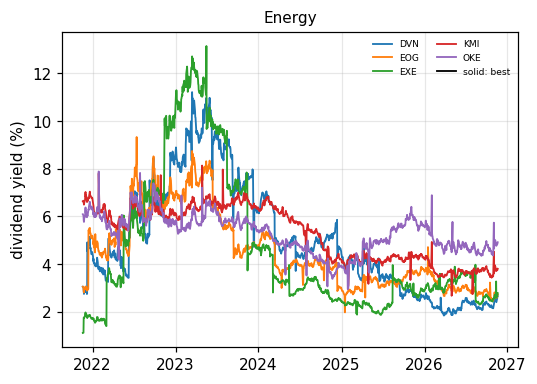
\includegraphics[width=\linewidth]{dividend_yield/best_energy.png}
\caption{Energy}
\end{subfigure}\hfill
\begin{subfigure}[t]{0.480\textwidth}
\centering
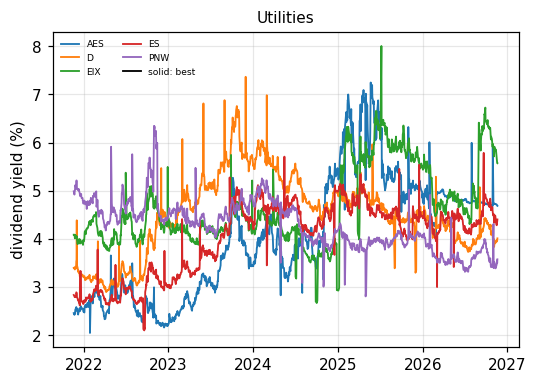
\includegraphics[width=\linewidth]{dividend_yield/best_utilities.png}
\caption{Utilities}
\end{subfigure}\hfill
\caption{The two sectors with the highest median yield over the last 5 years, (a) Energy and (b) Utilities, with their 5 highest-yielding companies; percent.}
\end{figure}
\begin{figure}[H]
\centering
\begin{subfigure}[t]{0.480\textwidth}
\centering
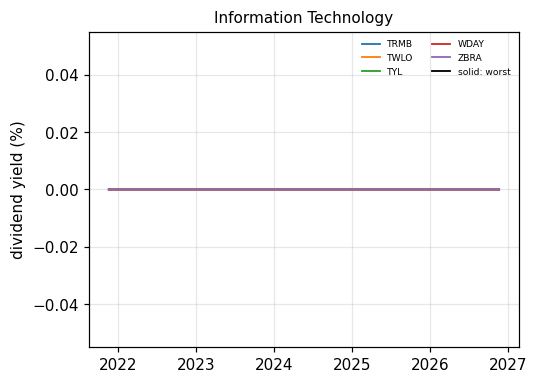
\includegraphics[width=\linewidth]{dividend_yield/worst_information_technology.png}
\caption{Information Technology}
\end{subfigure}\hfill
\begin{subfigure}[t]{0.480\textwidth}
\centering
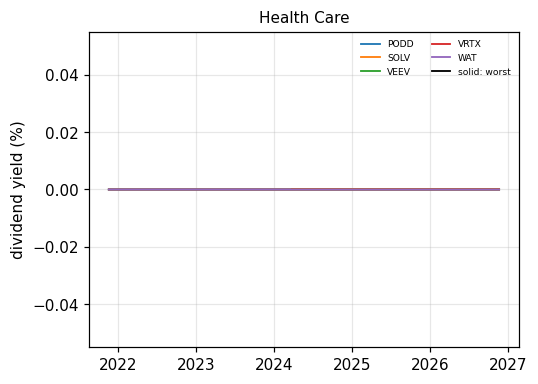
\includegraphics[width=\linewidth]{dividend_yield/worst_health_care.png}
\caption{Health Care}
\end{subfigure}\hfill
\caption{The two sectors with the lowest median yield, (a) Information Technology and (b) Health Care, with their 5 lowest-yielding companies; percent.}
\end{figure}
\newpage
\appendix
\section{Tickers and company names}
\label{app:tickers}
The companies analysed, by GICS sector, sorted by ticker. Tickers follow Yahoo Finance (a dash for a share class, as in BF-B).

\subsection{Communication Services}
\begin{table}[H]
\centering
\small
\begin{tabular}{lp{11cm}}
\hline
Ticker & Company \\
\hline
APP & AppLovin \\
CHTR & Charter Communications \\
CMCSA & Comcast \\
DIS & Walt Disney Company (The) \\
ECHO & EchoStar \\
FOX & Fox Corporation (Class B) \\
FOXA & Fox Corporation (Class A) \\
GOOG & Alphabet Inc. (Class C) \\
GOOGL & Alphabet Inc. (Class A) \\
LYV & Live Nation Entertainment \\
META & Meta Platforms \\
NFLX & Netflix \\
NWS & News Corp (Class B) \\
NWSA & News Corp (Class A) \\
OMC & Omnicom Group \\
RDDT & Reddit \\
SKYD & Skydance \\
T & AT\&T \\
TKO & TKO Group Holdings \\
TMUS & T-Mobile US \\
TTWO & Take-Two Interactive \\
VZ & Verizon \\
\hline
\end{tabular}
\end{table}
\subsection{Consumer Discretionary}
{\small
\begin{longtable}{lp{11cm}}
\hline
Ticker & Company \\
\hline
\endhead
ABNB & Airbnb \\
AMZN & Amazon \\
APTV & Aptiv \\
AZO & AutoZone \\
BBY & Best Buy \\
BKNG & Booking Holdings \\
CCL & Carnival Corporation \\
CMG & Chipotle Mexican Grill \\
CVNA & Carvana \\
DASH & DoorDash \\
DECK & Deckers Brands \\
DHI & D. R. Horton \\
DPZ & Domino's \\
DRI & Darden Restaurants \\
EBAY & eBay Inc. \\
EXPE & Expedia Group \\
F & Ford Motor Company \\
GM & General Motors \\
GPC & Genuine Parts Company \\
GRMN & Garmin \\
HAS & Hasbro \\
HD & Home Depot (The) \\
HLT & Hilton Worldwide \\
LEN & Lennar \\
LOW & Lowe's \\
LULU & Lululemon Athletica \\
LVS & Las Vegas Sands \\
MAR & Marriott International \\
MCD & McDonald's \\
MGM & MGM Resorts \\
NCLH & Norwegian Cruise Line Holdings \\
NKE & Nike, Inc. \\
NVR & NVR, Inc. \\
ORLY & O'Reilly Automotive \\
PHM & PulteGroup \\
RCL & Royal Caribbean Group \\
RL & Ralph Lauren Corporation \\
ROST & Ross Stores \\
SBUX & Starbucks \\
TJX & TJX Companies \\
TPR & Tapestry, Inc. \\
TSCO & Tractor Supply \\
TSLA & Tesla, Inc. \\
ULTA & Ulta Beauty \\
WSM & Williams-Sonoma, Inc. \\
WYNN & Wynn Resorts \\
YUM & Yum! Brands \\
\hline
\end{longtable}}
\subsection{Consumer Staples}
\begin{table}[H]
\centering
\small
\begin{tabular}{lp{11cm}}
\hline
Ticker & Company \\
\hline
ADM & Archer Daniels Midland \\
BF-B & Brown–Forman \\
BG & Bunge Global \\
CASY & Casey's \\
CHD & Church \& Dwight \\
CL & Colgate-Palmolive \\
CLX & Clorox \\
COST & Costco \\
DG & Dollar General \\
DLTR & Dollar Tree \\
EL & Estée Lauder Companies (The) \\
GIS & General Mills \\
HRL & Hormel Foods \\
HSY & Hershey Company (The) \\
KDP & Keurig Dr Pepper \\
KHC & Kraft Heinz \\
KMB & Kimberly-Clark \\
KO & Coca-Cola Company (The) \\
KR & Kroger \\
MDLZ & Mondelez International \\
MKC & McCormick \& Company \\
MNST & Monster Beverage \\
MO & Altria \\
PEP & PepsiCo \\
PG & Procter \& Gamble \\
PM & Philip Morris International \\
SJM & J.M. Smucker Company (The) \\
STZ & Constellation Brands \\
SYY & Sysco \\
TGT & Target Corporation \\
TSN & Tyson Foods \\
VYLR & Vylor \\
WMT & Walmart \\
\hline
\end{tabular}
\end{table}
\subsection{Energy}
\begin{table}[H]
\centering
\small
\begin{tabular}{lp{11cm}}
\hline
Ticker & Company \\
\hline
APA & APA Corporation \\
BKR & Baker Hughes \\
COP & ConocoPhillips \\
CVX & Chevron Corporation \\
DVN & Devon Energy \\
EOG & EOG Resources \\
EQT & EQT Corporation \\
EXE & Expand Energy \\
FANG & Diamondback Energy \\
HAL & Halliburton \\
KMI & Kinder Morgan \\
MPC & Marathon Petroleum \\
OKE & Oneok \\
OXY & Occidental Petroleum \\
PSX & Phillips 66 \\
SLB & Schlumberger \\
TPL & Texas Pacific Land Corporation \\
TRGP & Targa Resources \\
VLO & Valero Energy \\
WMB & Williams Companies \\
XOM & ExxonMobil \\
\hline
\end{tabular}
\end{table}
\subsection{Health Care}
{\small
\begin{longtable}{lp{11cm}}
\hline
Ticker & Company \\
\hline
\endhead
A & Agilent Technologies \\
ABBV & AbbVie \\
ABT & Abbott Laboratories \\
ALGN & Align Technology \\
AMGN & Amgen \\
BAX & Baxter International \\
BDX & Becton Dickinson \\
BIIB & Biogen \\
BMY & Bristol Myers Squibb \\
BSX & Boston Scientific \\
CAH & Cardinal Health \\
CI & Cigna \\
CNC & Centene Corporation \\
COO & Cooper Companies (The) \\
COR & Cencora \\
CRL & Charles River Laboratories \\
CVS & CVS Health \\
DGX & Quest Diagnostics \\
DHR & Danaher Corporation \\
DVA & DaVita \\
DXCM & Dexcom \\
ELV & Elevance Health \\
EW & Edwards Lifesciences \\
GEHC & GE HealthCare \\
GILD & Gilead Sciences \\
HCA & HCA Healthcare \\
HSIC & Henry Schein \\
HUM & Humana \\
IDXX & Idexx Laboratories \\
ILMN & Illumina, Inc. \\
INCY & Incyte \\
IQV & IQVIA \\
ISRG & Intuitive Surgical \\
JNJ & Johnson \& Johnson \\
LH & Labcorp \\
LLY & Lilly (Eli) \\
MCK & McKesson \\
MDT & Medtronic \\
MRK & Merck \& Co. \\
MRNA & Moderna \\
MTD & Mettler Toledo \\
PFE & Pfizer \\
PODD & Insulet Corporation \\
REGN & Regeneron Pharmaceuticals \\
RMD & ResMed \\
RVTY & Revvity \\
SOLV & Solventum \\
STE & Steris \\
SYK & Stryker Corporation \\
TECH & Bio-Techne \\
TMO & Thermo Fisher Scientific \\
UHS & Universal Health Services \\
UNH & UnitedHealth Group \\
VEEV & Veeva Systems \\
VRTX & Vertex Pharmaceuticals \\
VTRS & Viatris \\
WAT & Waters Corporation \\
WST & West Pharmaceutical Services \\
ZBH & Zimmer Biomet \\
ZTS & Zoetis \\
\hline
\end{longtable}}
\subsection{Industrials}
{\small
\begin{longtable}{lp{11cm}}
\hline
Ticker & Company \\
\hline
\endhead
ADP & Automatic Data Processing \\
ALLE & Allegion \\
AME & Ametek \\
AOS & A. O. Smith \\
AXON & Axon Enterprise \\
BA & Boeing \\
BE & Bloom Energy \\
BR & Broadridge Financial Solutions \\
CARR & Carrier Global \\
CAT & Caterpillar Inc. \\
CHRW & C.H. Robinson \\
CMI & Cummins \\
CPRT & Copart \\
CSX & CSX Corporation \\
CTAS & Cintas \\
DAL & Delta Air Lines \\
DD & DuPont \\
DE & Deere \& Company \\
DOV & Dover Corporation \\
EFX & Equifax \\
EME & Emcor \\
EMR & Emerson Electric \\
ETN & Eaton Corporation \\
EXPD & Expeditors International \\
FAST & Fastenal \\
FDX & FedEx \\
FDXF & FedEx Freight \\
FERG & Ferguson Enterprises \\
FIX & Comfort Systems USA \\
FTV & Fortive \\
GD & General Dynamics \\
GE & GE Aerospace \\
GEV & GE Vernova \\
GNRC & Generac \\
GWW & W. W. Grainger \\
HII & Huntington Ingalls Industries \\
HON & Honeywell Technologies \\
HONA & Honeywell Aerospace \\
HUBB & Hubbell Incorporated \\
HWM & Howmet Aerospace \\
IEX & IDEX Corporation \\
IR & Ingersoll Rand \\
ITW & Illinois Tool Works \\
J & Jacobs Solutions \\
JBHT & J.B. Hunt \\
JCI & Johnson Controls \\
LDOS & Leidos \\
LHX & L3Harris \\
LII & Lennox International \\
LMT & Lockheed Martin \\
LUV & Southwest Airlines \\
MAS & Masco \\
MMM & 3M \\
NDSN & Nordson Corporation \\
NOC & Northrop Grumman \\
NSC & Norfolk Southern \\
ODFL & Old Dominion \\
OTIS & Otis Worldwide \\
PAYX & Paychex \\
PCAR & Paccar \\
PH & Parker Hannifin \\
PNR & Pentair \\
PWR & Quanta Services \\
ROK & Rockwell Automation \\
ROL & Rollins, Inc. \\
RSG & Republic Services \\
RTX & RTX Corporation \\
SNA & Snap-on \\
SWK & Stanley Black \& Decker \\
TDG & TransDigm Group \\
TT & Trane Technologies \\
TXT & Textron \\
UAL & United Airlines Holdings \\
UBER & Uber \\
UNP & Union Pacific Corporation \\
UPS & United Parcel Service \\
URI & United Rentals \\
VLTO & Veralto \\
VRSK & Verisk Analytics \\
VRT & Vertiv \\
WAB & Wabtec \\
WM & Waste Management \\
XYL & Xylem Inc. \\
\hline
\end{longtable}}
\subsection{Information Technology}
{\small
\begin{longtable}{lp{11cm}}
\hline
Ticker & Company \\
\hline
\endhead
AAPL & Apple Inc. \\
ACN & Accenture \\
ADBE & Adobe Inc. \\
ADI & Analog Devices \\
ADSK & Autodesk \\
AKAM & Akamai Technologies \\
AMAT & Applied Materials \\
AMD & Advanced Micro Devices \\
ANET & Arista Networks \\
APH & Amphenol \\
AVGO & Broadcom \\
CDNS & Cadence Design Systems \\
CDW & CDW Corporation \\
CIEN & Ciena \\
COHR & Coherent Corp. \\
CRM & Salesforce \\
CRWD & CrowdStrike \\
CSCO & Cisco \\
CTSH & Cognizant \\
DDOG & Datadog \\
DELL & Dell Technologies \\
FFIV & F5, Inc. \\
FICO & Fair Isaac \\
FLEX & Flex Ltd. \\
FSLR & First Solar \\
FTNT & Fortinet \\
GDDY & GoDaddy \\
GEN & Gen Digital \\
GLW & Corning Inc. \\
HPE & Hewlett Packard Enterprise \\
HPQ & HP Inc. \\
IBM & IBM \\
INTC & Intel \\
INTU & Intuit \\
IT & Gartner \\
JBL & Jabil \\
KEYS & Keysight Technologies \\
KLAC & KLA Corporation \\
LITE & Lumentum \\
LRCX & Lam Research \\
MCHP & Microchip Technology \\
MPWR & Monolithic Power Systems \\
MRVL & Marvell Technology \\
MSFT & Microsoft \\
MSI & Motorola Solutions \\
MU & Micron Technology \\
NOW & ServiceNow \\
NTAP & NetApp \\
NVDA & Nvidia \\
NXPI & NXP Semiconductors \\
OKTA & Okta, Inc. \\
ON & ON Semiconductor \\
ORCL & Oracle Corporation \\
P & Everpure \\
PANW & Palo Alto Networks \\
PLTR & Palantir Technologies \\
PTC & PTC Inc. \\
Q & Qnity Electronics \\
QCOM & Qualcomm \\
ROP & Roper Technologies \\
SMCI & Supermicro \\
SNDK & Sandisk \\
SNPS & Synopsys \\
STX & Seagate Technology \\
SWKS & Skyworks Solutions \\
TDY & Teledyne Technologies \\
TEL & TE Connectivity \\
TER & Teradyne \\
TRMB & Trimble Inc. \\
TWLO & Twilio \\
TXN & Texas Instruments \\
TYL & Tyler Technologies \\
VRSN & Verisign \\
WDAY & Workday, Inc. \\
WDC & Western Digital \\
ZBRA & Zebra Technologies \\
\hline
\end{longtable}}
\subsection{Materials}
\begin{table}[H]
\centering
\small
\begin{tabular}{lp{11cm}}
\hline
Ticker & Company \\
\hline
ALB & Albemarle Corporation \\
AMCR & Amcor \\
APD & Air Products \\
AVY & Avery Dennison \\
BALL & Ball Corporation \\
CF & CF Industries \\
CRH & CRH plc \\
DOW & Dow Inc. \\
ECL & Ecolab \\
FCX & Freeport-McMoRan \\
IFF & International Flavors \& Fragrances \\
IP & International Paper \\
LIN & Linde plc \\
LYB & LyondellBasell \\
MLM & Martin Marietta Materials \\
MOS & Mosaic Company (The) \\
NEM & Newmont \\
NUE & Nucor \\
PKG & Packaging Corporation of America \\
PPG & PPG Industries \\
SHW & Sherwin-Williams \\
STLD & Steel Dynamics \\
SW & Smurfit Westrock \\
VMC & Vulcan Materials Company \\
\hline
\end{tabular}
\end{table}
\subsection{Utilities}
\begin{table}[H]
\centering
\small
\begin{tabular}{lp{11cm}}
\hline
Ticker & Company \\
\hline
AEE & Ameren \\
AEP & American Electric Power \\
AES & AES Corporation \\
ATO & Atmos Energy \\
AWK & American Water Works \\
CEG & Constellation Energy \\
CMS & CMS Energy \\
CNP & CenterPoint Energy \\
D & Dominion Energy \\
DTE & DTE Energy \\
DUK & Duke Energy \\
ED & Consolidated Edison \\
EIX & Edison International \\
ES & Eversource Energy \\
ETR & Entergy \\
EVRG & Evergy \\
EXC & Exelon \\
FE & FirstEnergy \\
LNT & Alliant Energy \\
NEE & NextEra Energy \\
NI & NiSource \\
NRG & NRG Energy \\
PCG & PG\&E Corporation \\
PEG & Public Service Enterprise Group \\
PNW & Pinnacle West Capital \\
PPL & PPL Corporation \\
SO & Southern Company \\
SRE & Sempra \\
VST & Vistra Corp. \\
WEC & WEC Energy Group \\
XEL & Xcel Energy \\
\hline
\end{tabular}
\end{table}
\section{Fundamentals: full history per sector}
\label{app:fundamentals}
For every GICS sector, the revenue of its companies with the highest (solid) and lowest (dashed) annualised revenue growth over all years in the data.

\subsection{Communication Services}
\begin{figure}[H]
\centering
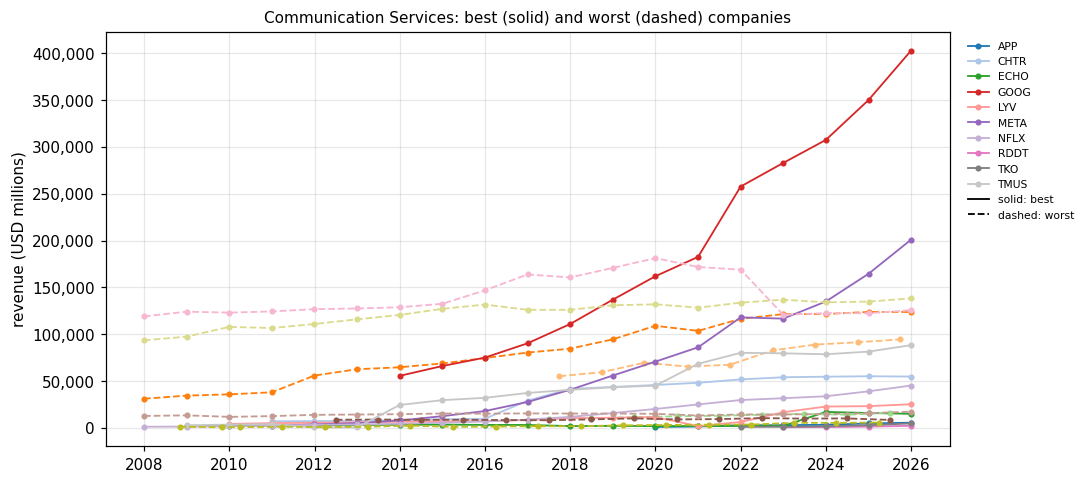
\includegraphics[width=1\textwidth]{appendix/fundamentals/communication_services.png}
\caption{Communication Services: annual revenue of the 10 companies with the highest (solid) and lowest (dashed) revenue growth over the full history; USD millions.}
\end{figure}
\subsection{Consumer Discretionary}
\begin{figure}[H]
\centering
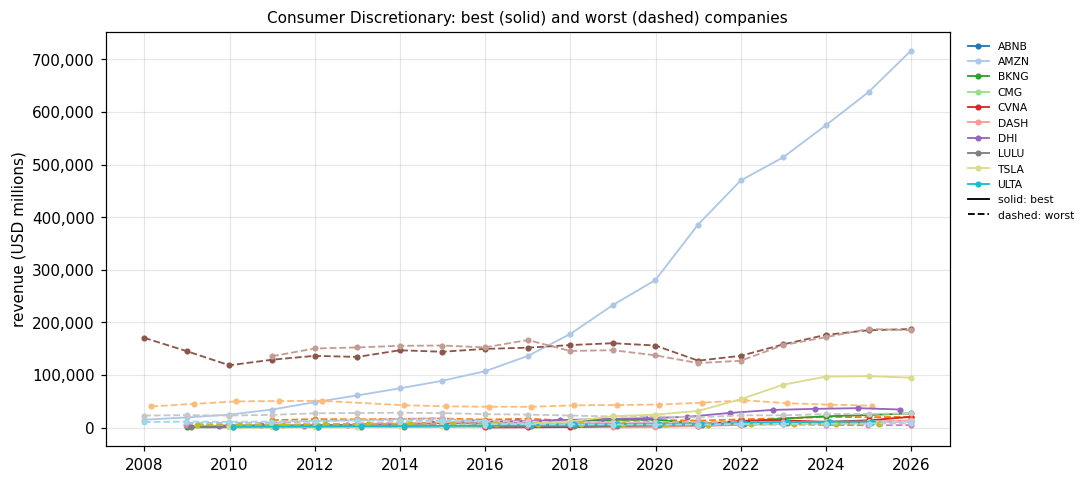
\includegraphics[width=1\textwidth]{appendix/fundamentals/consumer_discretionary.png}
\caption{Consumer Discretionary: annual revenue of the 10 companies with the highest (solid) and lowest (dashed) revenue growth over the full history; USD millions.}
\end{figure}
\subsection{Consumer Staples}
\begin{figure}[H]
\centering
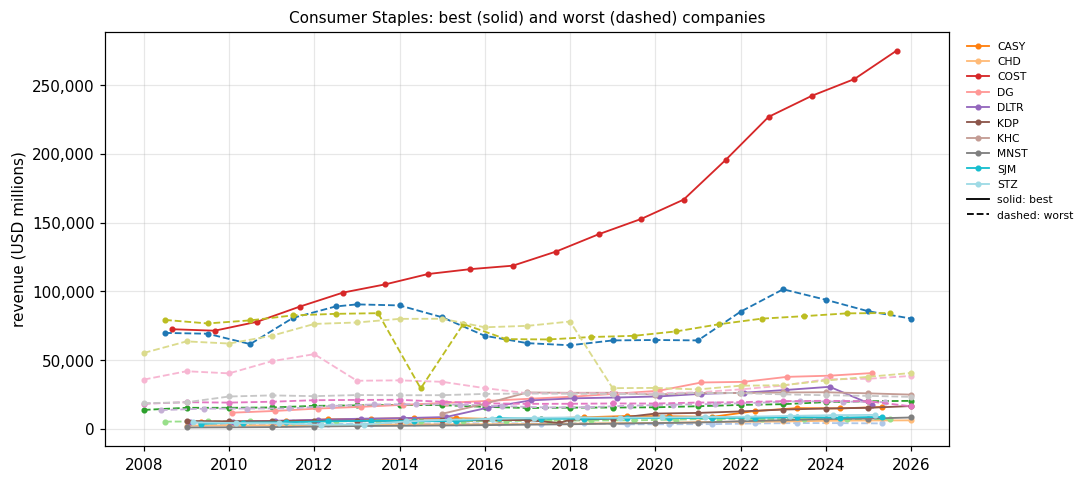
\includegraphics[width=1\textwidth]{appendix/fundamentals/consumer_staples.png}
\caption{Consumer Staples: annual revenue of the 10 companies with the highest (solid) and lowest (dashed) revenue growth over the full history; USD millions.}
\end{figure}
\subsection{Energy}
\begin{figure}[H]
\centering
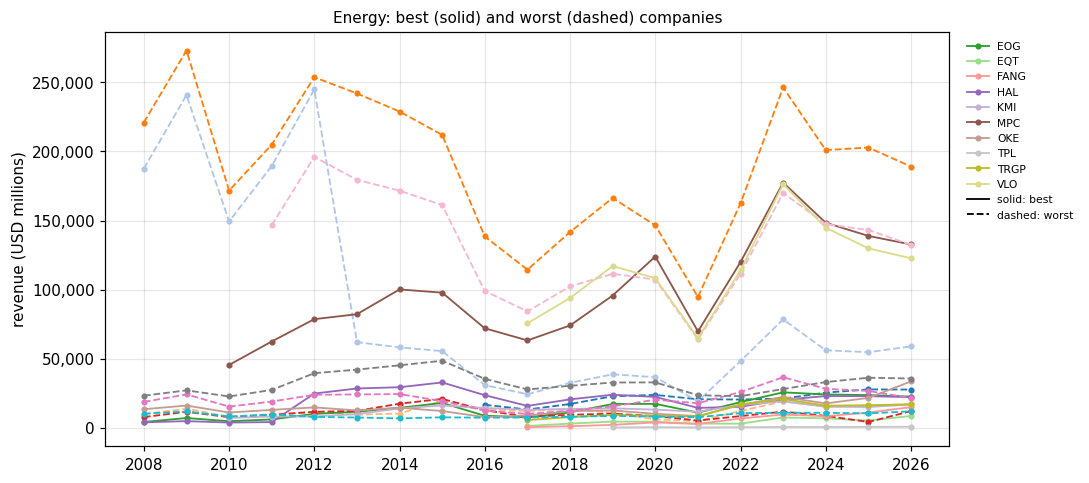
\includegraphics[width=1\textwidth]{appendix/fundamentals/energy.png}
\caption{Energy: annual revenue of the 10 companies with the highest (solid) and lowest (dashed) revenue growth over the full history; USD millions.}
\end{figure}
\subsection{Health Care}
\begin{figure}[H]
\centering
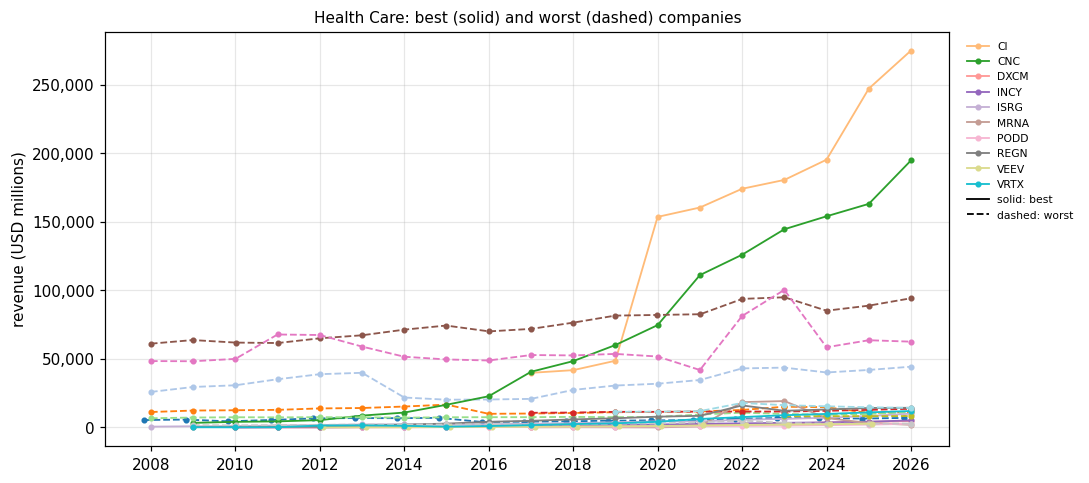
\includegraphics[width=1\textwidth]{appendix/fundamentals/health_care.png}
\caption{Health Care: annual revenue of the 10 companies with the highest (solid) and lowest (dashed) revenue growth over the full history; USD millions.}
\end{figure}
\subsection{Industrials}
\begin{figure}[H]
\centering
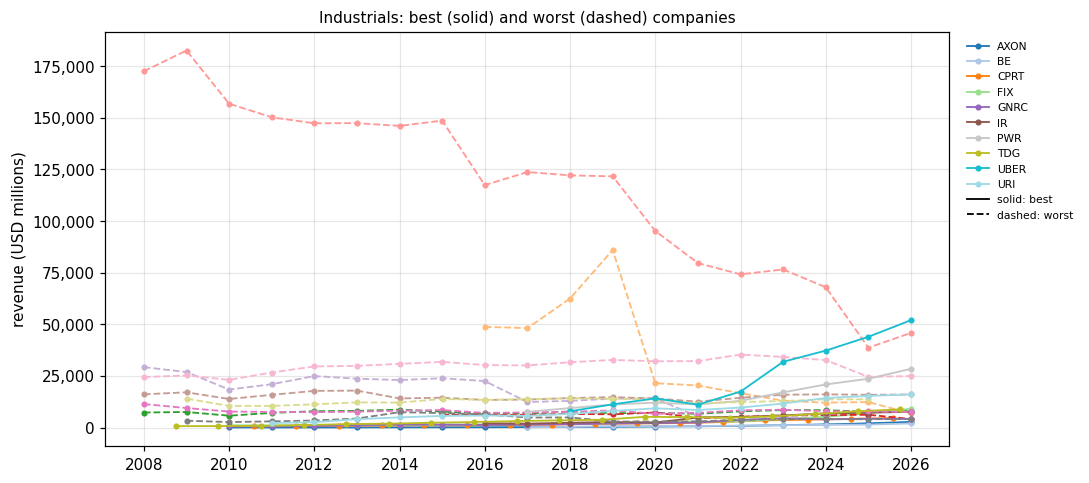
\includegraphics[width=1\textwidth]{appendix/fundamentals/industrials.png}
\caption{Industrials: annual revenue of the 10 companies with the highest (solid) and lowest (dashed) revenue growth over the full history; USD millions.}
\end{figure}
\subsection{Information Technology}
\begin{figure}[H]
\centering
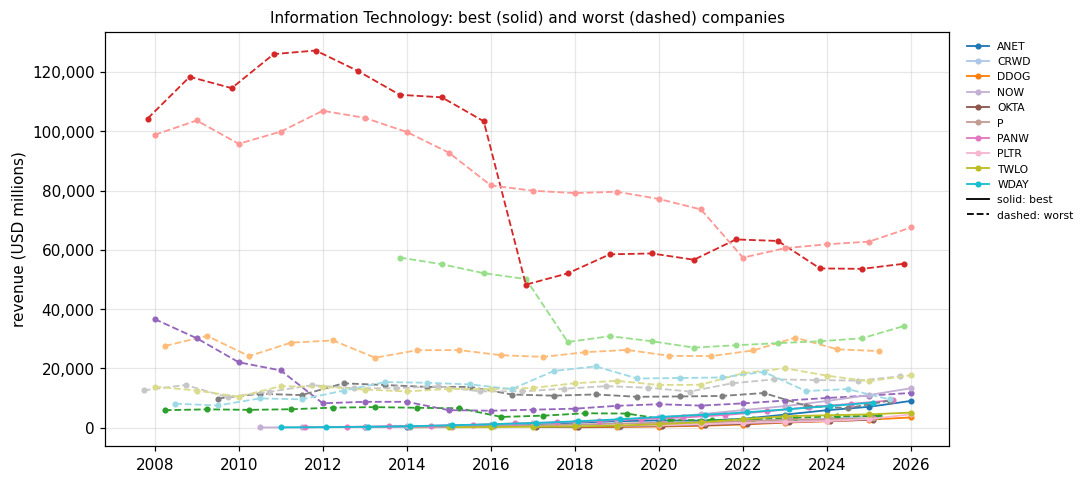
\includegraphics[width=1\textwidth]{appendix/fundamentals/information_technology.png}
\caption{Information Technology: annual revenue of the 10 companies with the highest (solid) and lowest (dashed) revenue growth over the full history; USD millions.}
\end{figure}
\subsection{Materials}
\begin{figure}[H]
\centering
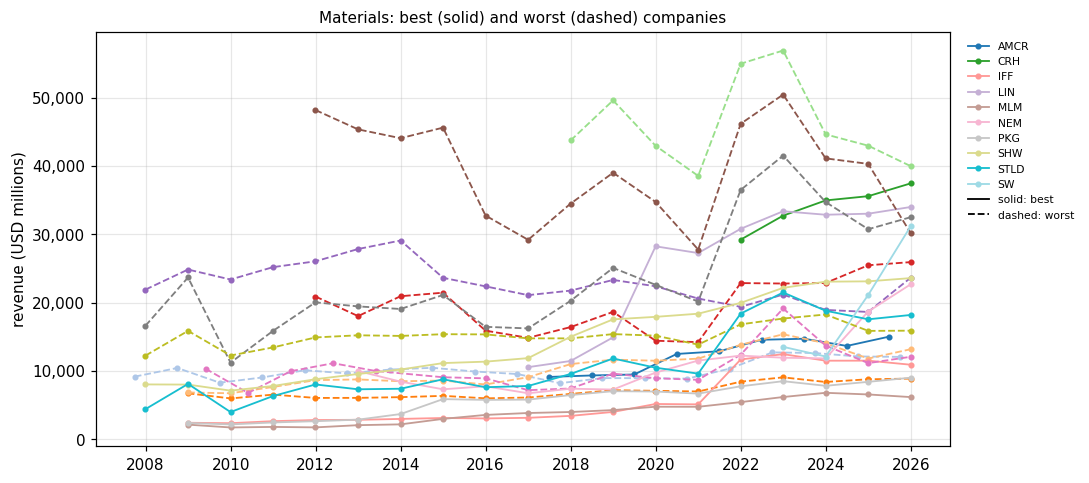
\includegraphics[width=1\textwidth]{appendix/fundamentals/materials.png}
\caption{Materials: annual revenue of the 10 companies with the highest (solid) and lowest (dashed) revenue growth over the full history; USD millions.}
\end{figure}
\subsection{Utilities}
\begin{figure}[H]
\centering
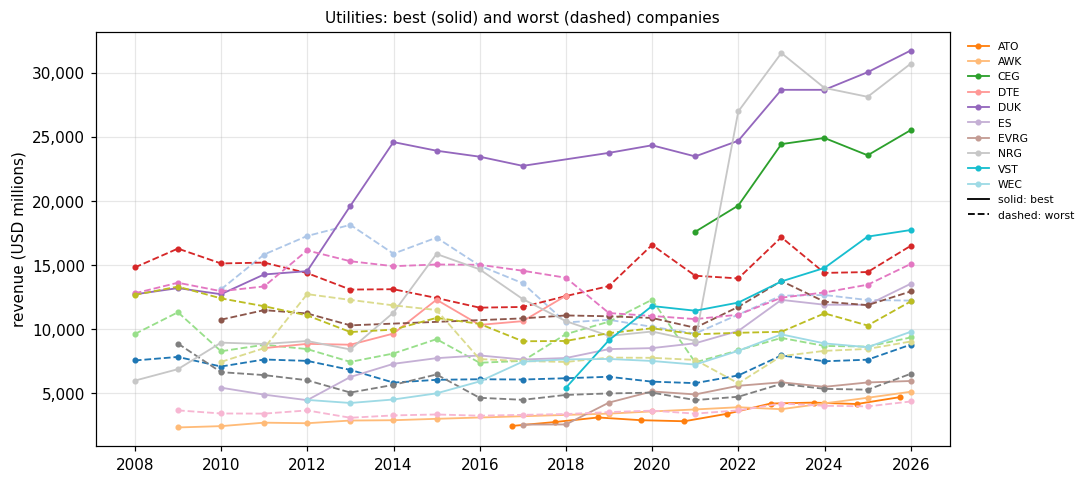
\includegraphics[width=1\textwidth]{appendix/fundamentals/utilities.png}
\caption{Utilities: annual revenue of the 10 companies with the highest (solid) and lowest (dashed) revenue growth over the full history; USD millions.}
\end{figure}
\section{Total return: full history per sector}
\label{app:total_return}
For every GICS sector, growth of 1 USD for its companies with the highest (solid) and lowest (dashed) annualised total return since each company's first date in the data (at least one year).

\subsection{Communication Services}
\begin{figure}[H]
\centering
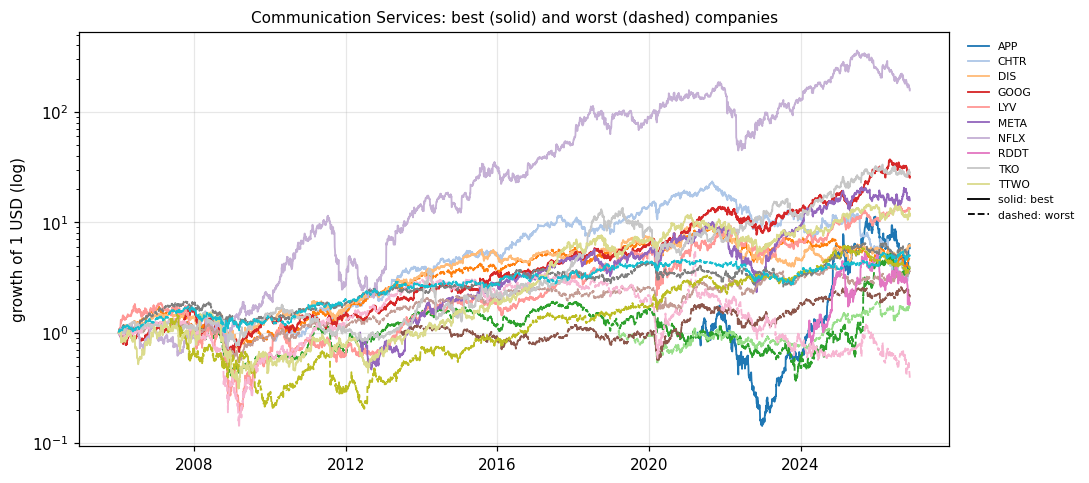
\includegraphics[width=1\textwidth]{appendix/total_return/communication_services.png}
\caption{Communication Services: growth of 1 USD for the 10 companies with the highest (solid) and lowest (dashed) total return over the full history; log scale.}
\end{figure}
\subsection{Consumer Discretionary}
\begin{figure}[H]
\centering
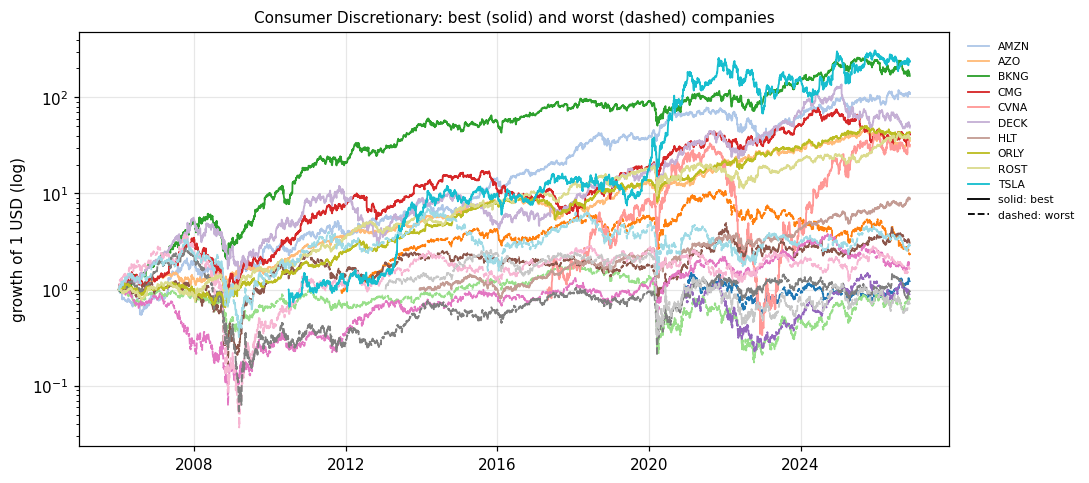
\includegraphics[width=1\textwidth]{appendix/total_return/consumer_discretionary.png}
\caption{Consumer Discretionary: growth of 1 USD for the 10 companies with the highest (solid) and lowest (dashed) total return over the full history; log scale.}
\end{figure}
\subsection{Consumer Staples}
\begin{figure}[H]
\centering
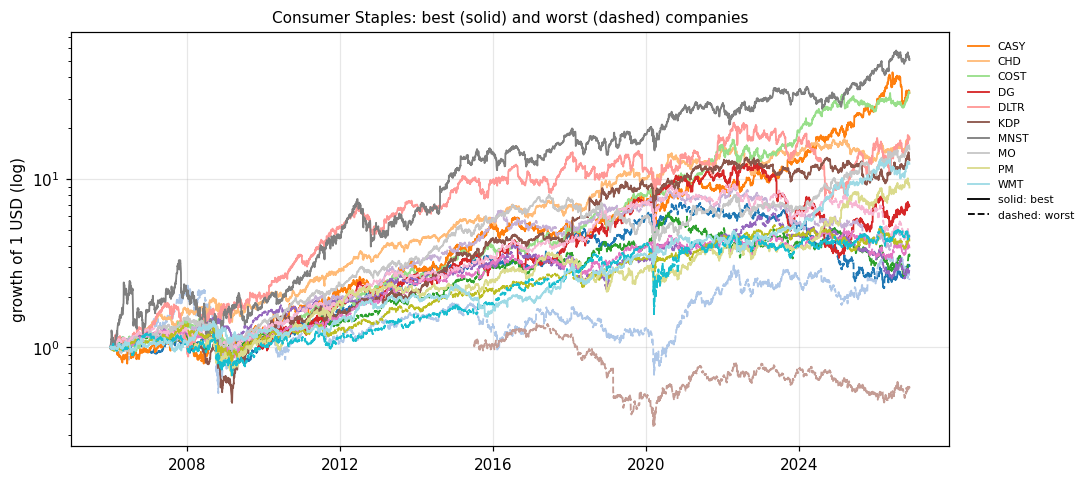
\includegraphics[width=1\textwidth]{appendix/total_return/consumer_staples.png}
\caption{Consumer Staples: growth of 1 USD for the 10 companies with the highest (solid) and lowest (dashed) total return over the full history; log scale.}
\end{figure}
\subsection{Energy}
\begin{figure}[H]
\centering
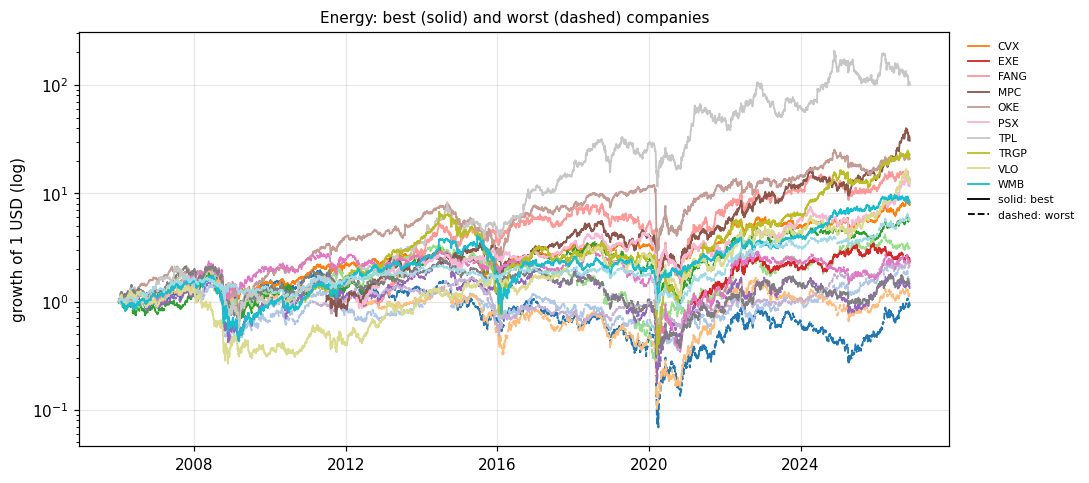
\includegraphics[width=1\textwidth]{appendix/total_return/energy.png}
\caption{Energy: growth of 1 USD for the 10 companies with the highest (solid) and lowest (dashed) total return over the full history; log scale.}
\end{figure}
\subsection{Health Care}
\begin{figure}[H]
\centering
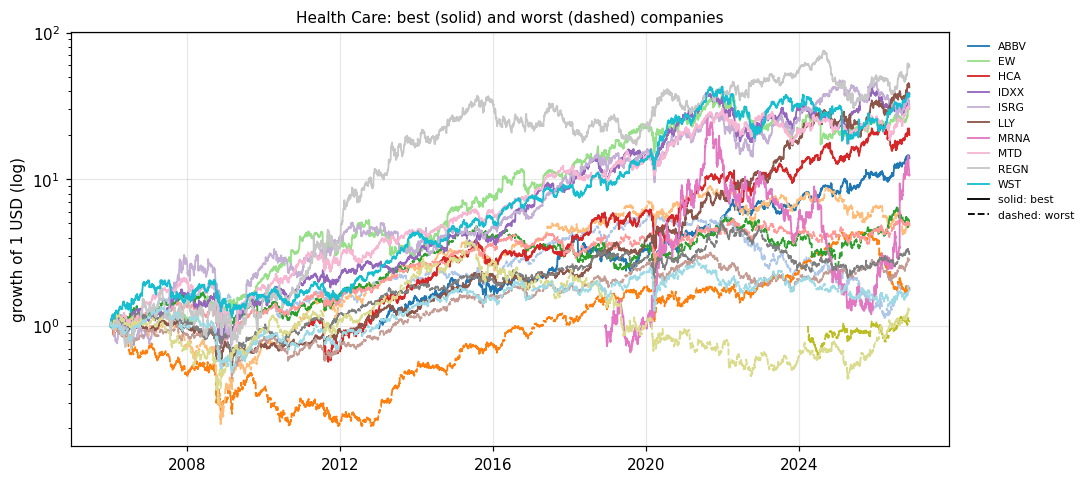
\includegraphics[width=1\textwidth]{appendix/total_return/health_care.png}
\caption{Health Care: growth of 1 USD for the 10 companies with the highest (solid) and lowest (dashed) total return over the full history; log scale.}
\end{figure}
\subsection{Industrials}
\begin{figure}[H]
\centering
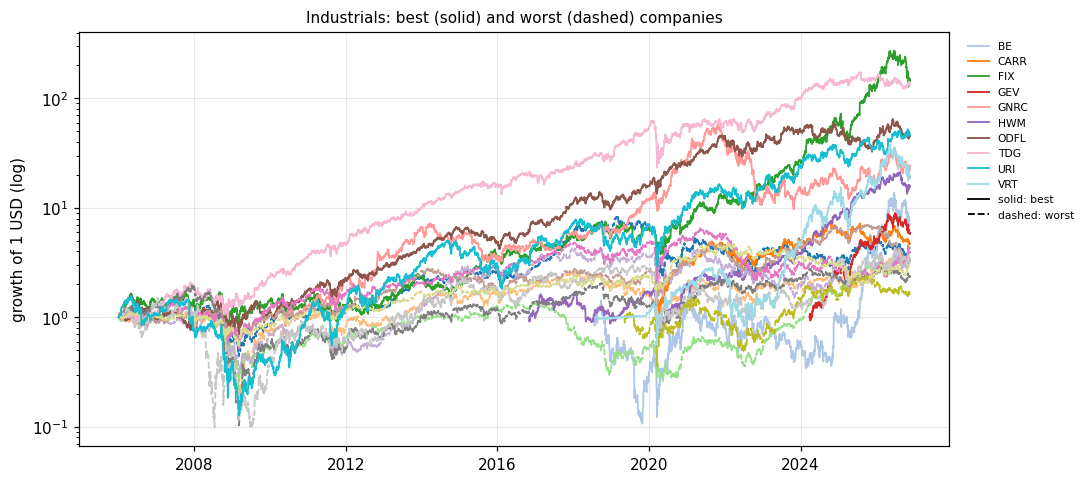
\includegraphics[width=1\textwidth]{appendix/total_return/industrials.png}
\caption{Industrials: growth of 1 USD for the 10 companies with the highest (solid) and lowest (dashed) total return over the full history; log scale.}
\end{figure}
\subsection{Information Technology}
\begin{figure}[H]
\centering
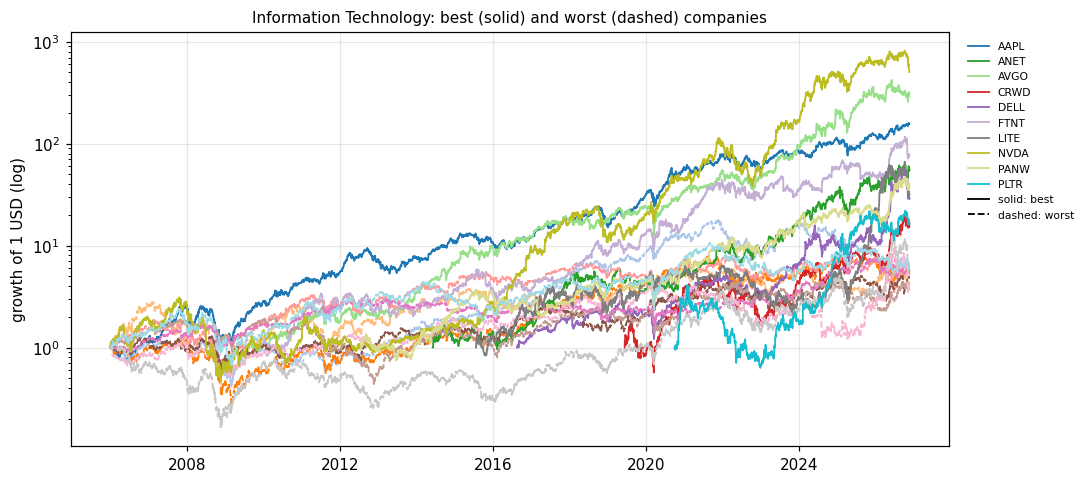
\includegraphics[width=1\textwidth]{appendix/total_return/information_technology.png}
\caption{Information Technology: growth of 1 USD for the 10 companies with the highest (solid) and lowest (dashed) total return over the full history; log scale.}
\end{figure}
\subsection{Materials}
\begin{figure}[H]
\centering
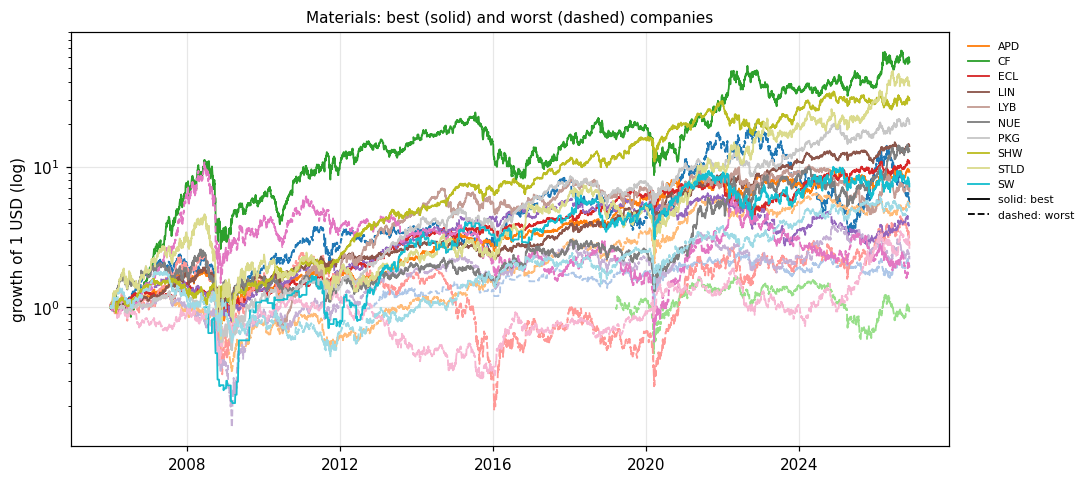
\includegraphics[width=1\textwidth]{appendix/total_return/materials.png}
\caption{Materials: growth of 1 USD for the 10 companies with the highest (solid) and lowest (dashed) total return over the full history; log scale.}
\end{figure}
\subsection{Utilities}
\begin{figure}[H]
\centering
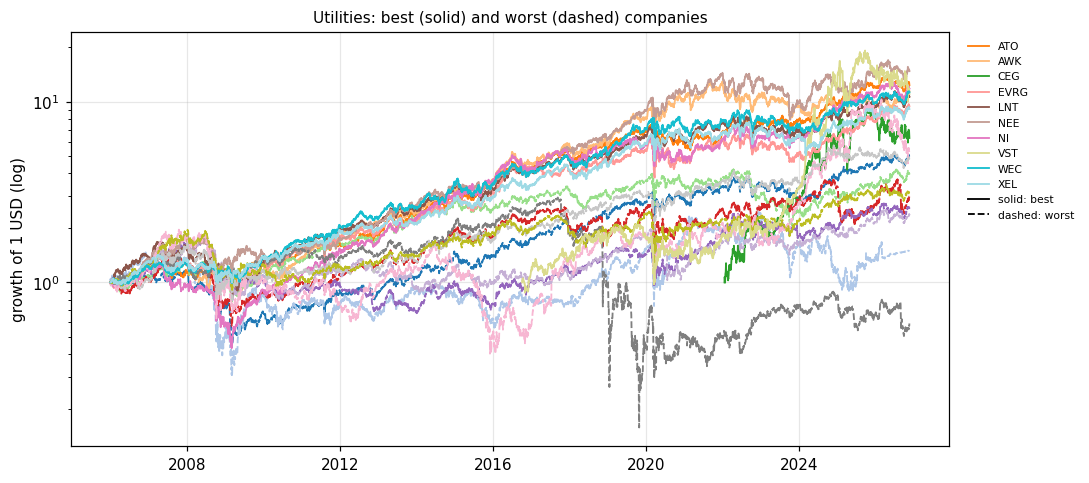
\includegraphics[width=1\textwidth]{appendix/total_return/utilities.png}
\caption{Utilities: growth of 1 USD for the 10 companies with the highest (solid) and lowest (dashed) total return over the full history; log scale.}
\end{figure}
\section{Relative return: full history per sector}
\label{app:relative_return}
For every GICS sector, growth relative to the sector fund for its companies that beat it most (solid) and trailed it most (dashed) over the full history.

\subsection{Communication Services}
\begin{figure}[H]
\centering
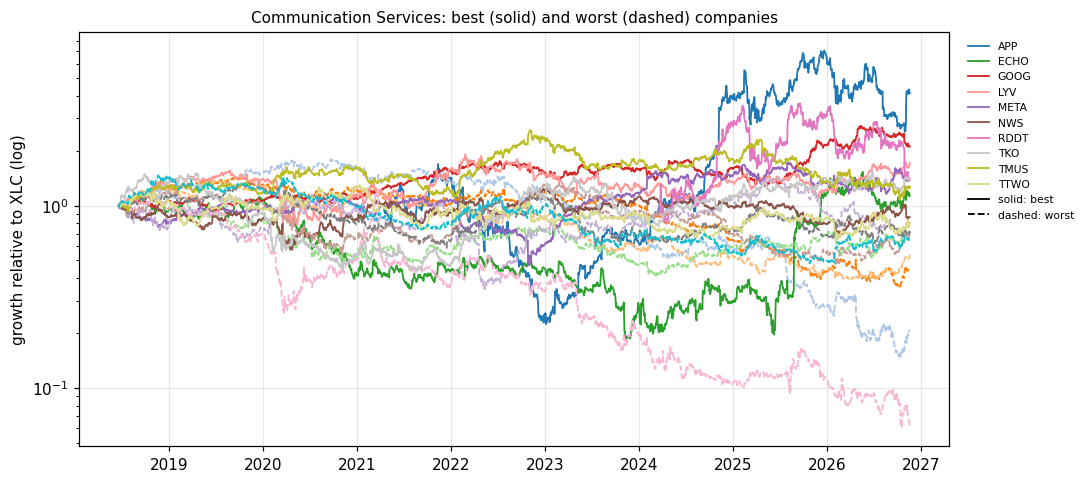
\includegraphics[width=1\textwidth]{appendix/relative_return/communication_services.png}
\caption{Communication Services: growth relative to XLC for the 10 companies with the highest (solid) and lowest (dashed) annualised relative return over the full history; log scale.}
\end{figure}
\subsection{Consumer Discretionary}
\begin{figure}[H]
\centering
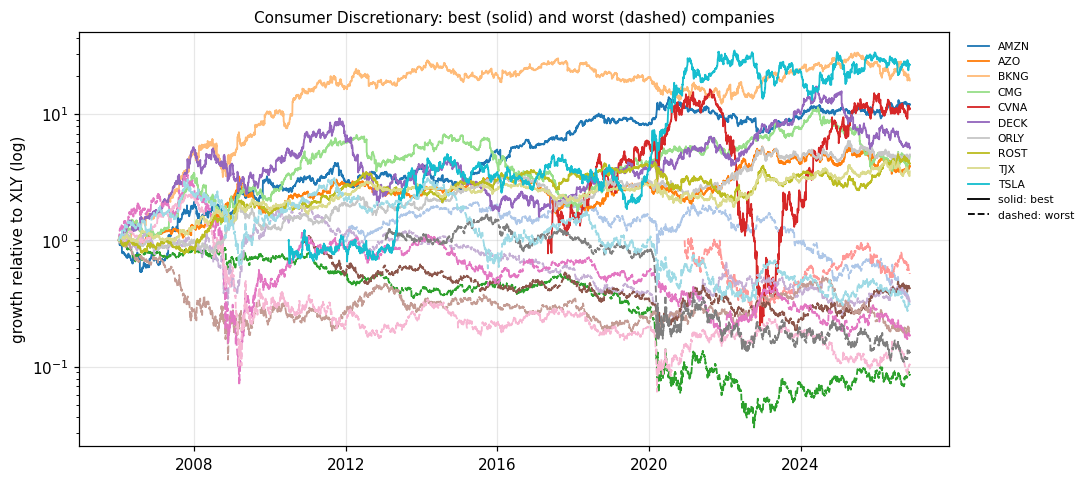
\includegraphics[width=1\textwidth]{appendix/relative_return/consumer_discretionary.png}
\caption{Consumer Discretionary: growth relative to XLY for the 10 companies with the highest (solid) and lowest (dashed) annualised relative return over the full history; log scale.}
\end{figure}
\subsection{Consumer Staples}
\begin{figure}[H]
\centering
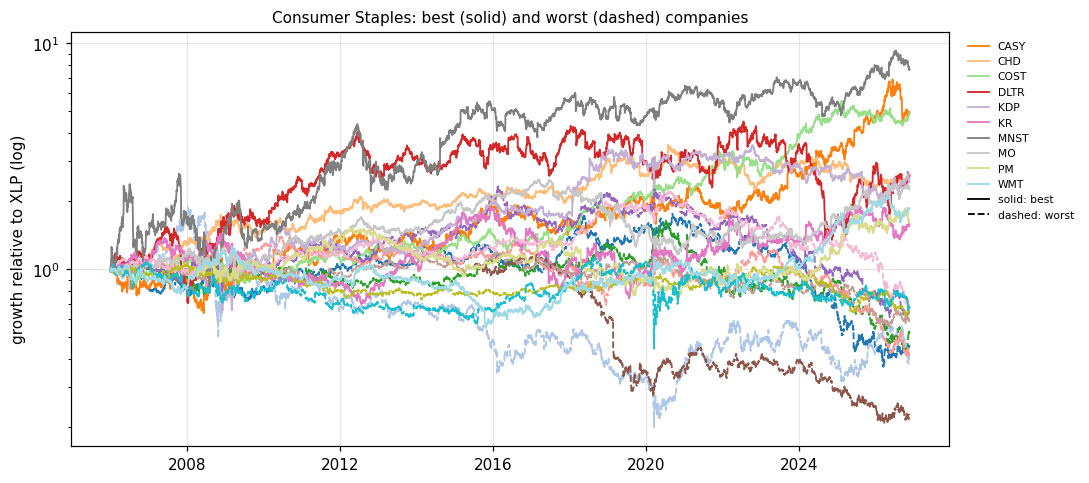
\includegraphics[width=1\textwidth]{appendix/relative_return/consumer_staples.png}
\caption{Consumer Staples: growth relative to XLP for the 10 companies with the highest (solid) and lowest (dashed) annualised relative return over the full history; log scale.}
\end{figure}
\subsection{Energy}
\begin{figure}[H]
\centering
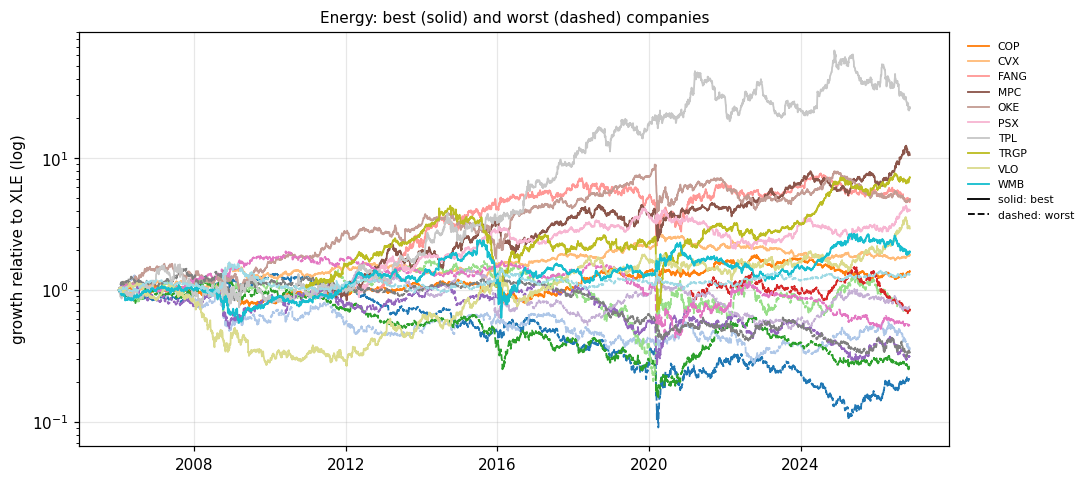
\includegraphics[width=1\textwidth]{appendix/relative_return/energy.png}
\caption{Energy: growth relative to XLE for the 10 companies with the highest (solid) and lowest (dashed) annualised relative return over the full history; log scale.}
\end{figure}
\subsection{Health Care}
\begin{figure}[H]
\centering
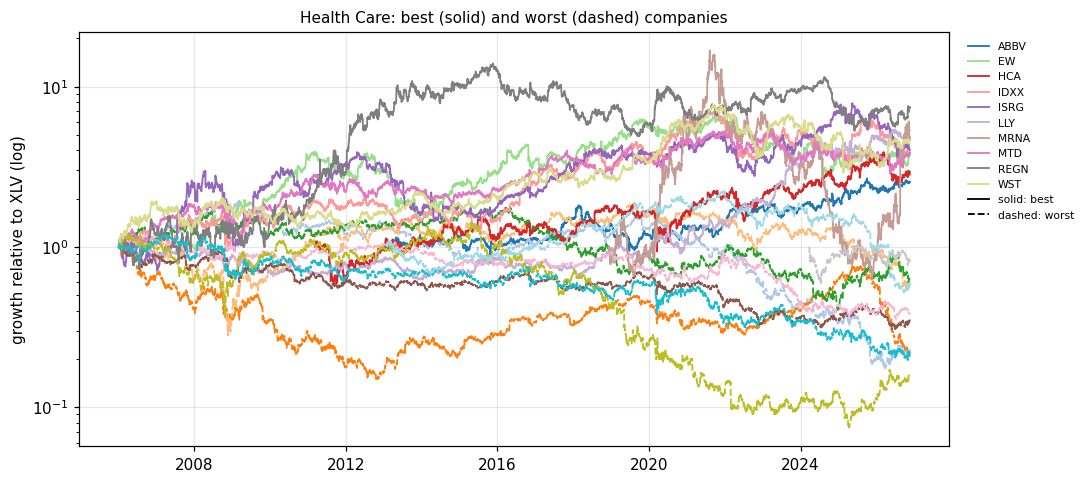
\includegraphics[width=1\textwidth]{appendix/relative_return/health_care.png}
\caption{Health Care: growth relative to XLV for the 10 companies with the highest (solid) and lowest (dashed) annualised relative return over the full history; log scale.}
\end{figure}
\subsection{Industrials}
\begin{figure}[H]
\centering
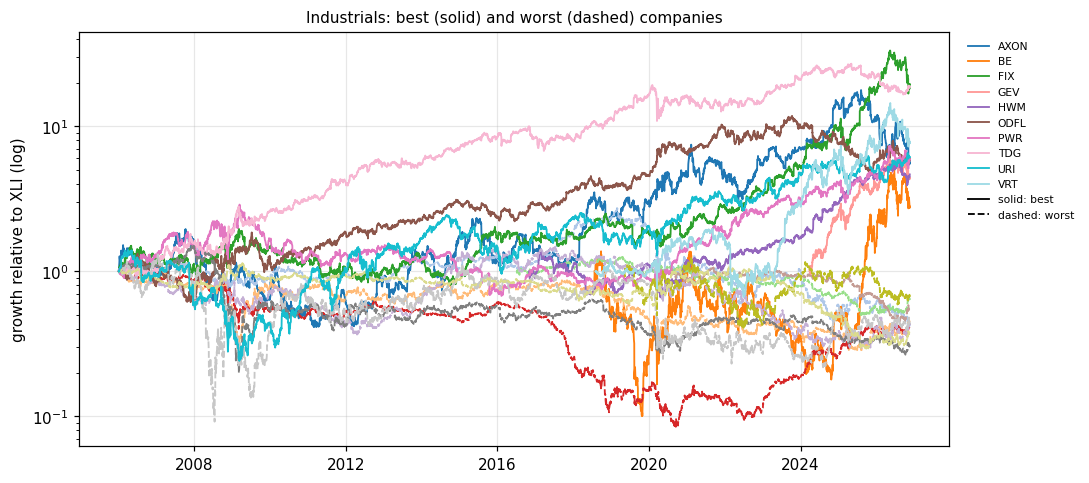
\includegraphics[width=1\textwidth]{appendix/relative_return/industrials.png}
\caption{Industrials: growth relative to XLI for the 10 companies with the highest (solid) and lowest (dashed) annualised relative return over the full history; log scale.}
\end{figure}
\subsection{Information Technology}
\begin{figure}[H]
\centering
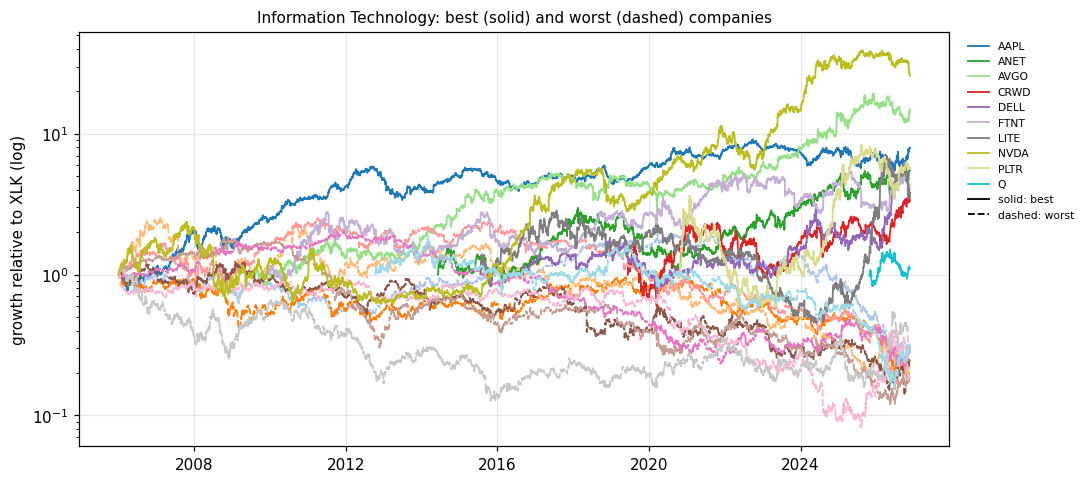
\includegraphics[width=1\textwidth]{appendix/relative_return/information_technology.png}
\caption{Information Technology: growth relative to XLK for the 10 companies with the highest (solid) and lowest (dashed) annualised relative return over the full history; log scale.}
\end{figure}
\subsection{Materials}
\begin{figure}[H]
\centering
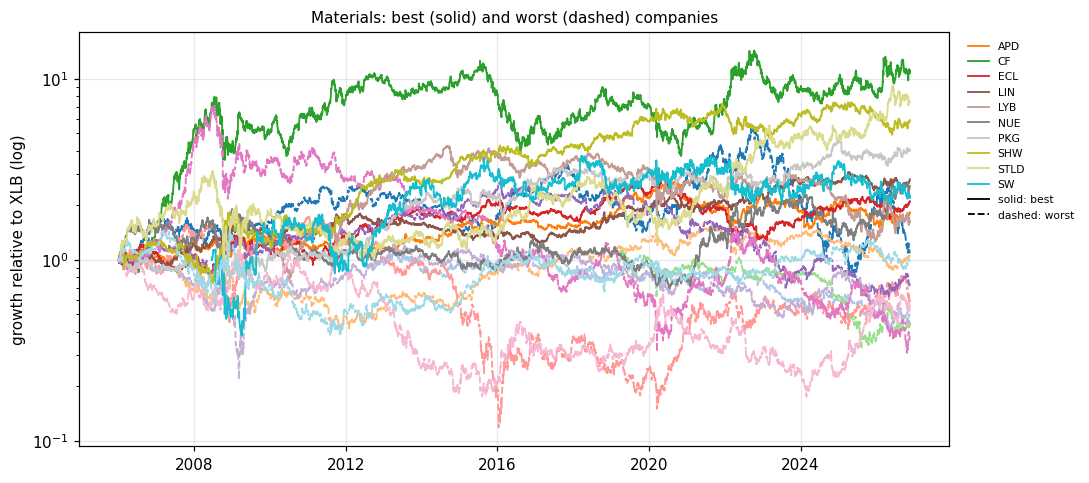
\includegraphics[width=1\textwidth]{appendix/relative_return/materials.png}
\caption{Materials: growth relative to XLB for the 10 companies with the highest (solid) and lowest (dashed) annualised relative return over the full history; log scale.}
\end{figure}
\subsection{Utilities}
\begin{figure}[H]
\centering
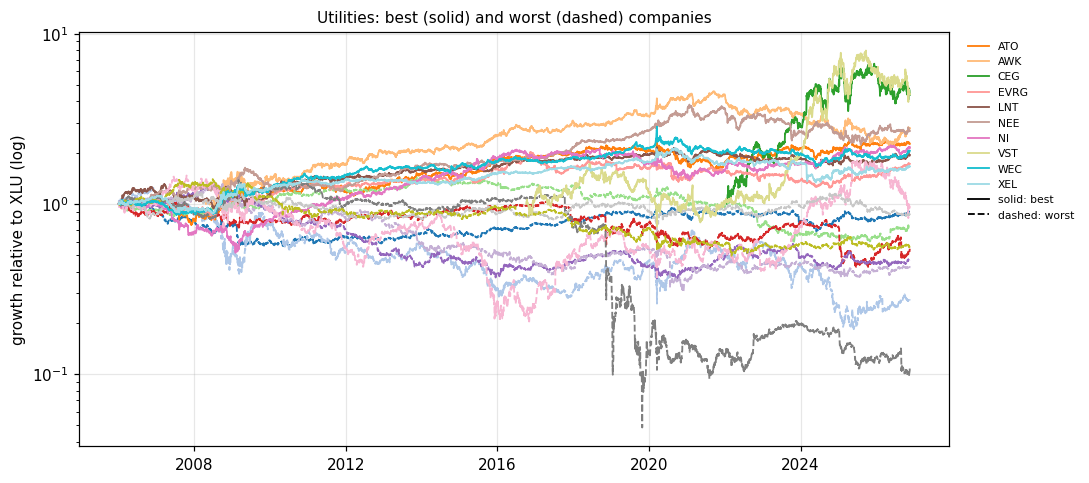
\includegraphics[width=1\textwidth]{appendix/relative_return/utilities.png}
\caption{Utilities: growth relative to XLU for the 10 companies with the highest (solid) and lowest (dashed) annualised relative return over the full history; log scale.}
\end{figure}
\section{P/E: full history per sector}
\label{app:pe}
For every GICS sector, the P/E of its companies with the lowest (solid) and highest (dashed) median P/E over the full history, and the lead-lag correlation of monthly P/E and price changes. P/E is price divided by earnings per share, so at lag 0 the two move together by construction; the other lags show whether P/E changes come before or after price changes.

\begin{figure}[H]
\centering
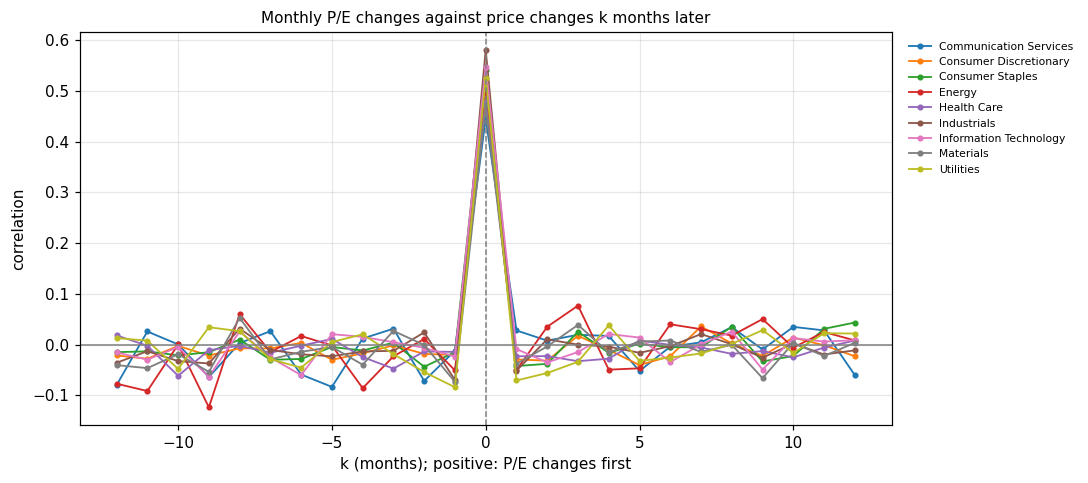
\includegraphics[width=1\textwidth]{appendix/pe/lead_lag.png}
\caption{Mean correlation, over each sector's companies, of monthly P/E changes with price changes k months later; positive k: the P/E changes first.}
\end{figure}
\subsection{Communication Services}
\begin{figure}[H]
\centering
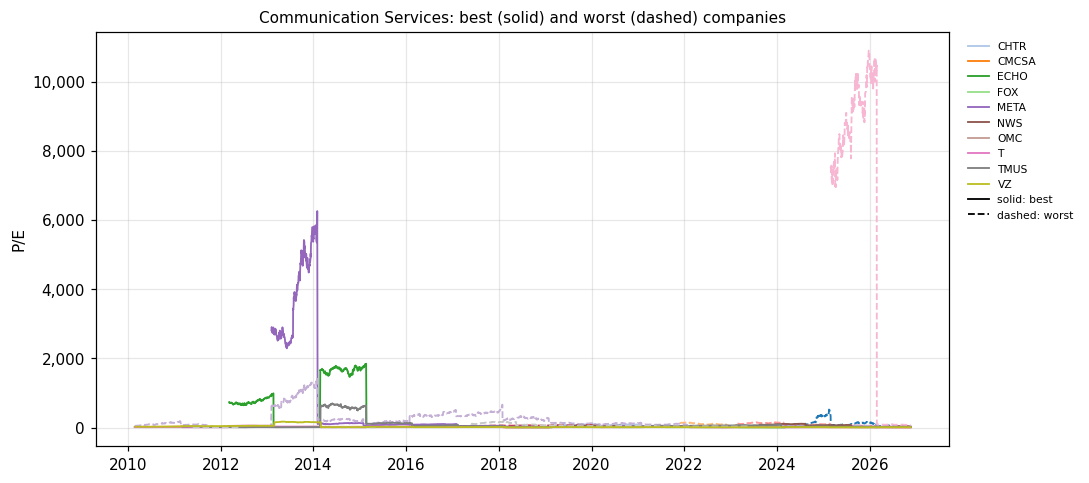
\includegraphics[width=1\textwidth]{appendix/pe/communication_services.png}
\caption{Communication Services: P/E of the 10 companies with the lowest (solid) and highest (dashed) median P/E over the full history.}
\end{figure}
\subsection{Consumer Discretionary}
\begin{figure}[H]
\centering
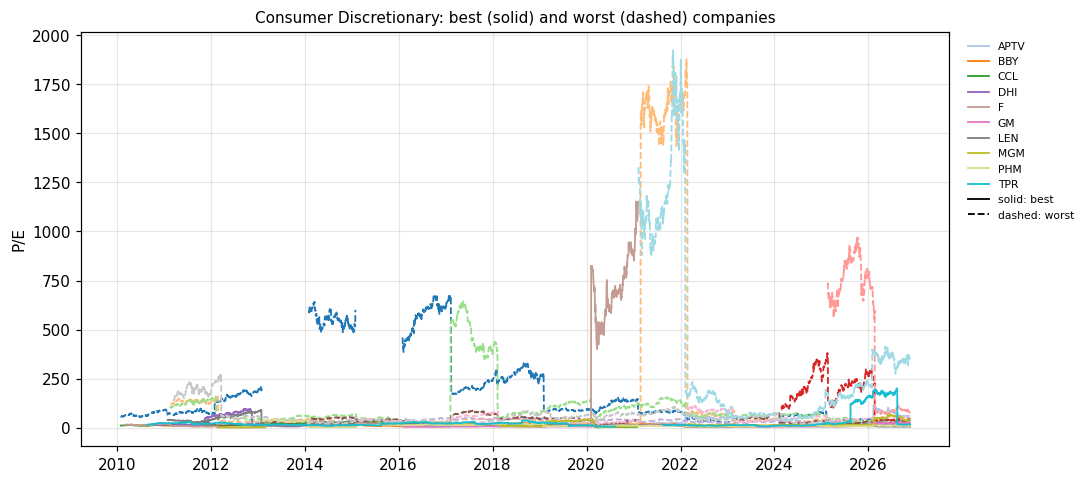
\includegraphics[width=1\textwidth]{appendix/pe/consumer_discretionary.png}
\caption{Consumer Discretionary: P/E of the 10 companies with the lowest (solid) and highest (dashed) median P/E over the full history.}
\end{figure}
\subsection{Consumer Staples}
\begin{figure}[H]
\centering
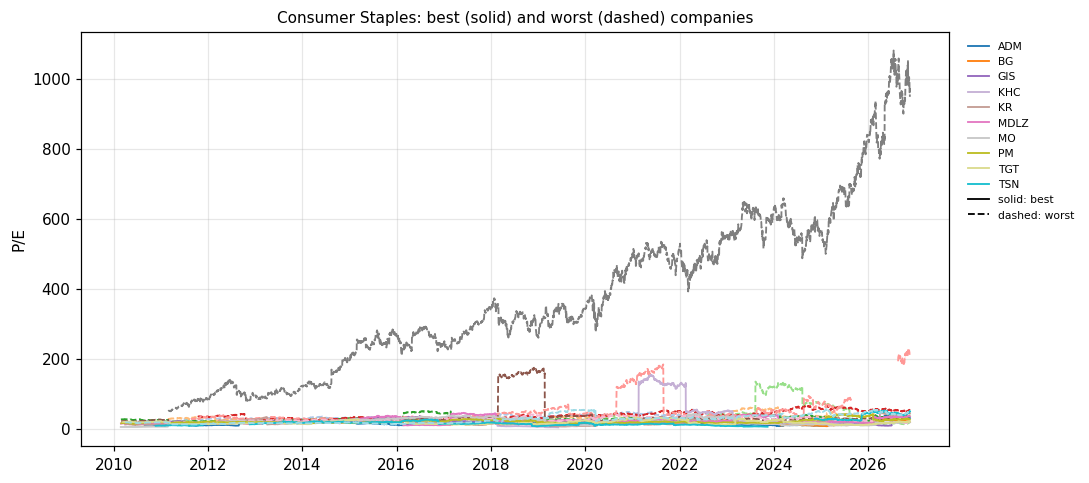
\includegraphics[width=1\textwidth]{appendix/pe/consumer_staples.png}
\caption{Consumer Staples: P/E of the 10 companies with the lowest (solid) and highest (dashed) median P/E over the full history.}
\end{figure}
\subsection{Energy}
\begin{figure}[H]
\centering
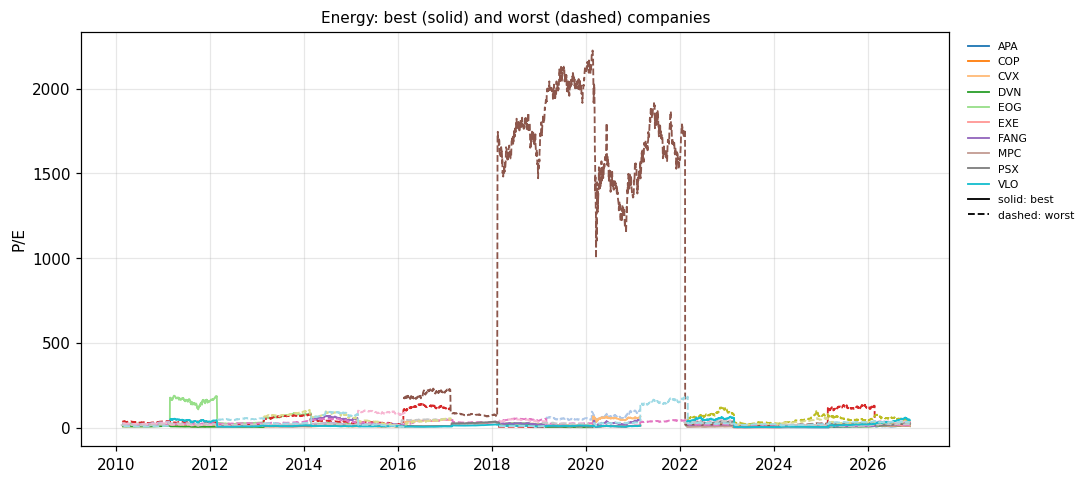
\includegraphics[width=1\textwidth]{appendix/pe/energy.png}
\caption{Energy: P/E of the 10 companies with the lowest (solid) and highest (dashed) median P/E over the full history.}
\end{figure}
\subsection{Health Care}
\begin{figure}[H]
\centering
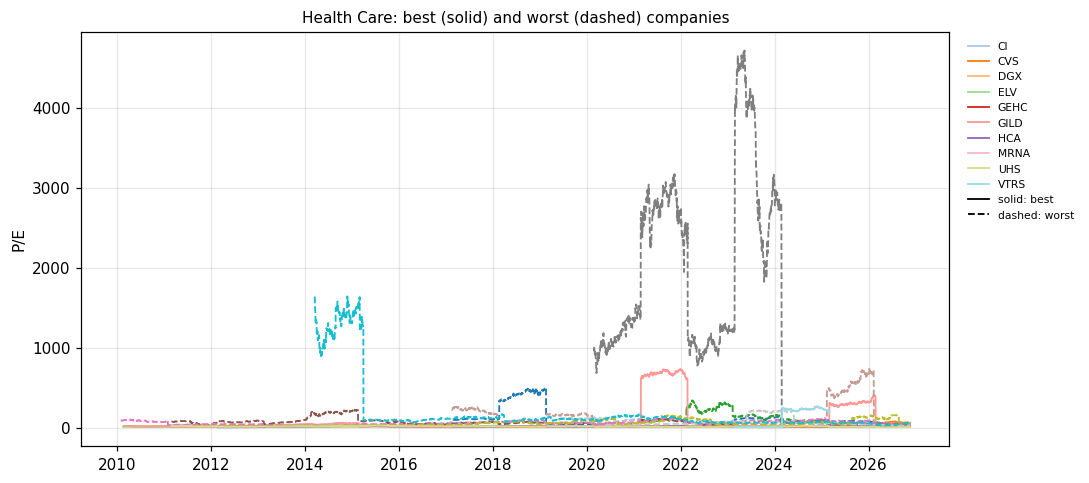
\includegraphics[width=1\textwidth]{appendix/pe/health_care.png}
\caption{Health Care: P/E of the 10 companies with the lowest (solid) and highest (dashed) median P/E over the full history.}
\end{figure}
\subsection{Industrials}
\begin{figure}[H]
\centering
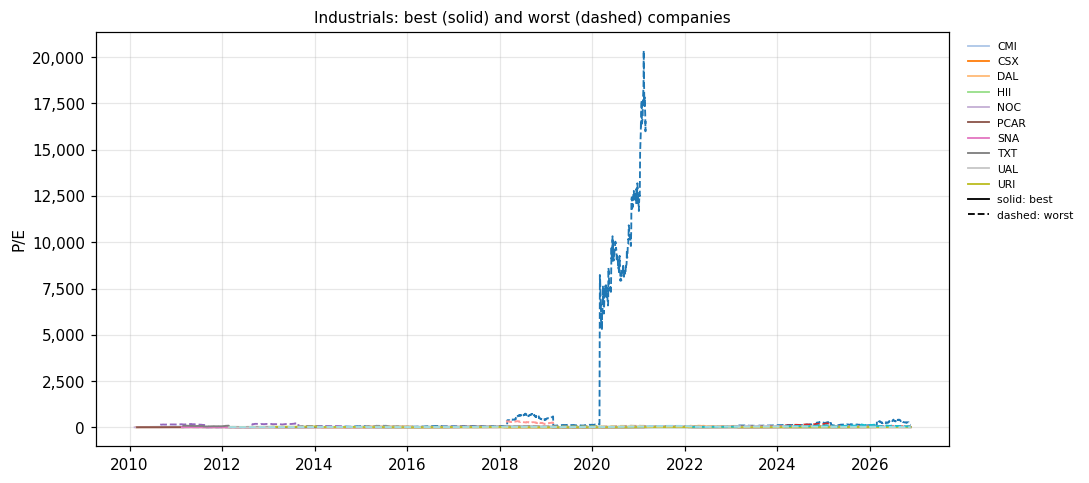
\includegraphics[width=1\textwidth]{appendix/pe/industrials.png}
\caption{Industrials: P/E of the 10 companies with the lowest (solid) and highest (dashed) median P/E over the full history.}
\end{figure}
\subsection{Information Technology}
\begin{figure}[H]
\centering
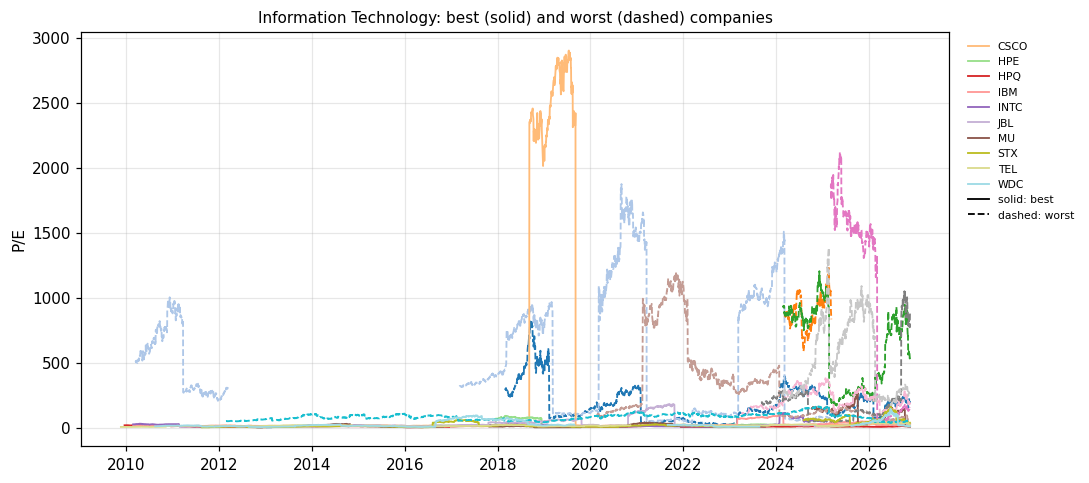
\includegraphics[width=1\textwidth]{appendix/pe/information_technology.png}
\caption{Information Technology: P/E of the 10 companies with the lowest (solid) and highest (dashed) median P/E over the full history.}
\end{figure}
\subsection{Materials}
\begin{figure}[H]
\centering
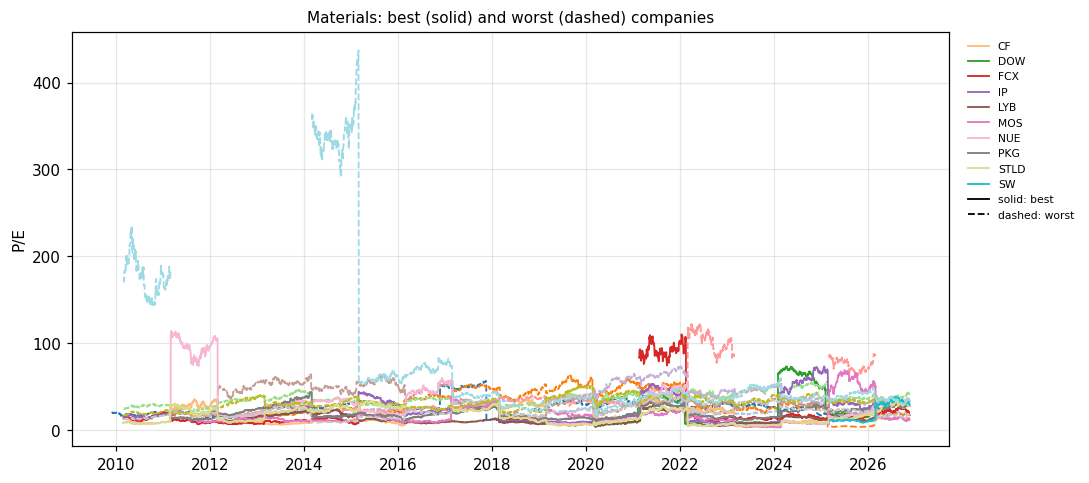
\includegraphics[width=1\textwidth]{appendix/pe/materials.png}
\caption{Materials: P/E of the 10 companies with the lowest (solid) and highest (dashed) median P/E over the full history.}
\end{figure}
\subsection{Utilities}
\begin{figure}[H]
\centering
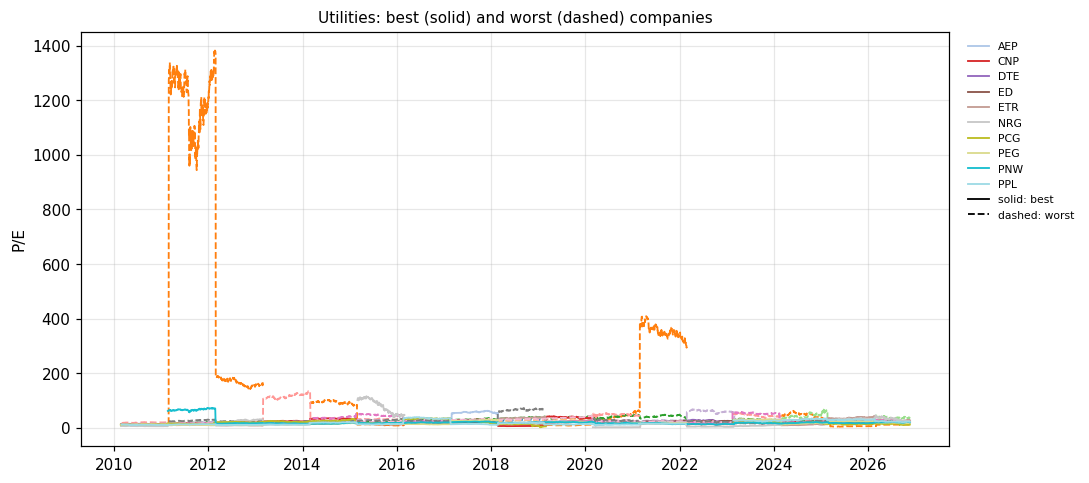
\includegraphics[width=1\textwidth]{appendix/pe/utilities.png}
\caption{Utilities: P/E of the 10 companies with the lowest (solid) and highest (dashed) median P/E over the full history.}
\end{figure}
\section{Dividend yield: full history per sector}
\label{app:dividend_yield}
For every GICS sector, the trailing dividend yield of its companies with the highest (solid) and lowest (dashed) mean yield over the full history.

\subsection{Communication Services}
\begin{figure}[H]
\centering
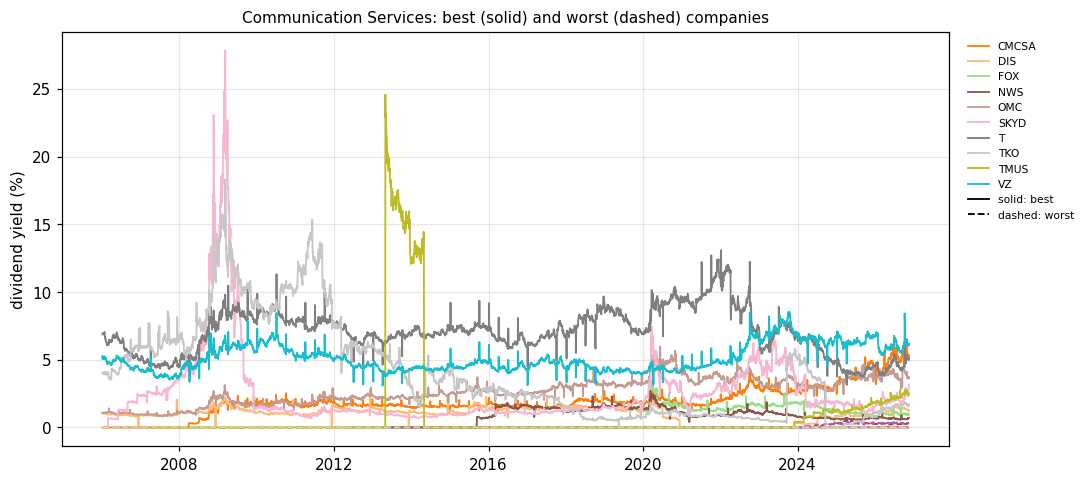
\includegraphics[width=1\textwidth]{appendix/dividend_yield/communication_services.png}
\caption{Communication Services: trailing dividend yield of the 10 companies with the highest (solid) and lowest (dashed) mean yield over the full history; percent.}
\end{figure}
\subsection{Consumer Discretionary}
\begin{figure}[H]
\centering
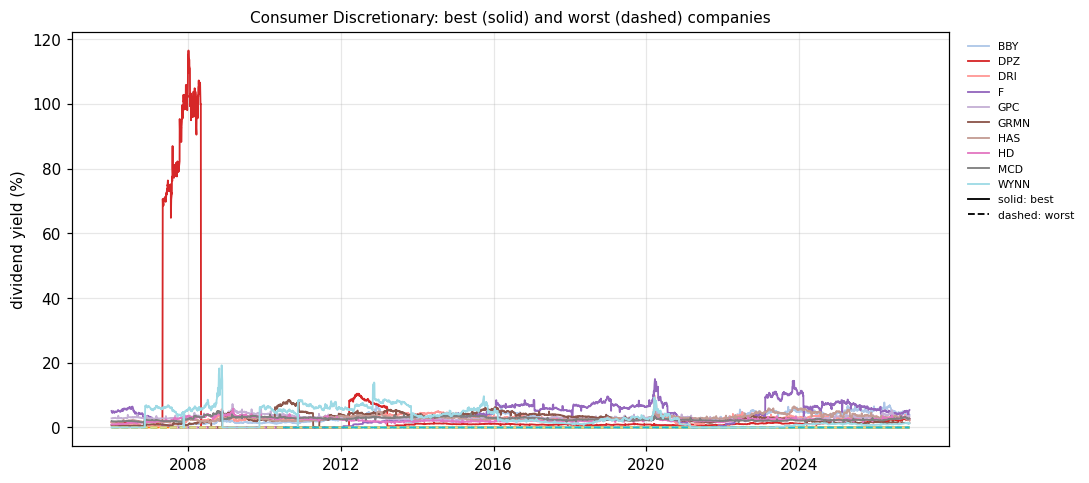
\includegraphics[width=1\textwidth]{appendix/dividend_yield/consumer_discretionary.png}
\caption{Consumer Discretionary: trailing dividend yield of the 10 companies with the highest (solid) and lowest (dashed) mean yield over the full history; percent.}
\end{figure}
\subsection{Consumer Staples}
\begin{figure}[H]
\centering
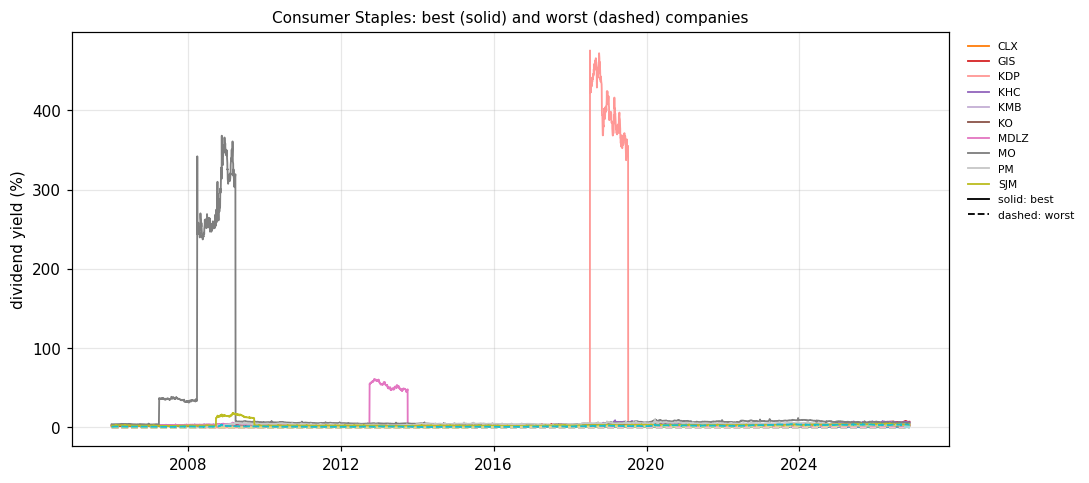
\includegraphics[width=1\textwidth]{appendix/dividend_yield/consumer_staples.png}
\caption{Consumer Staples: trailing dividend yield of the 10 companies with the highest (solid) and lowest (dashed) mean yield over the full history; percent.}
\end{figure}
\subsection{Energy}
\begin{figure}[H]
\centering
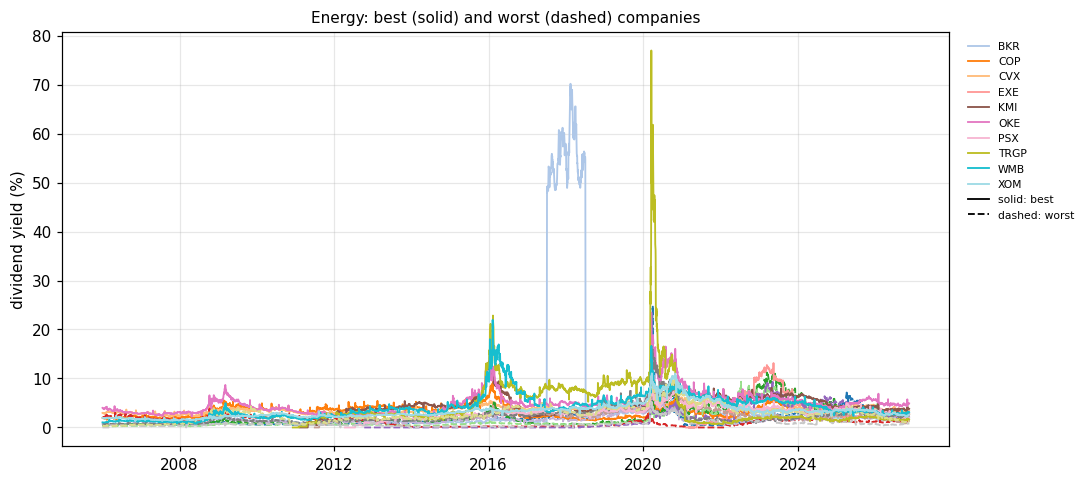
\includegraphics[width=1\textwidth]{appendix/dividend_yield/energy.png}
\caption{Energy: trailing dividend yield of the 10 companies with the highest (solid) and lowest (dashed) mean yield over the full history; percent.}
\end{figure}
\subsection{Health Care}
\begin{figure}[H]
\centering
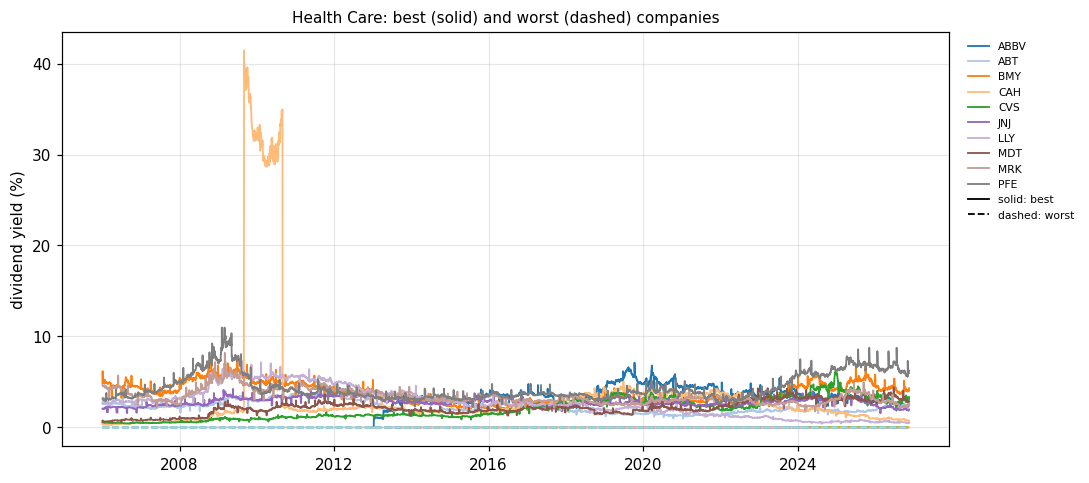
\includegraphics[width=1\textwidth]{appendix/dividend_yield/health_care.png}
\caption{Health Care: trailing dividend yield of the 10 companies with the highest (solid) and lowest (dashed) mean yield over the full history; percent.}
\end{figure}
\subsection{Industrials}
\begin{figure}[H]
\centering
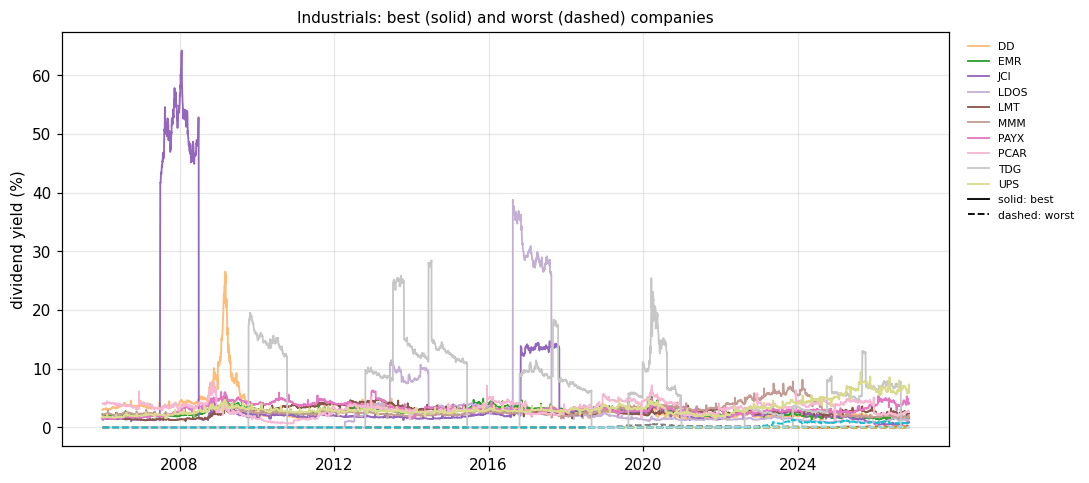
\includegraphics[width=1\textwidth]{appendix/dividend_yield/industrials.png}
\caption{Industrials: trailing dividend yield of the 10 companies with the highest (solid) and lowest (dashed) mean yield over the full history; percent.}
\end{figure}
\subsection{Information Technology}
\begin{figure}[H]
\centering
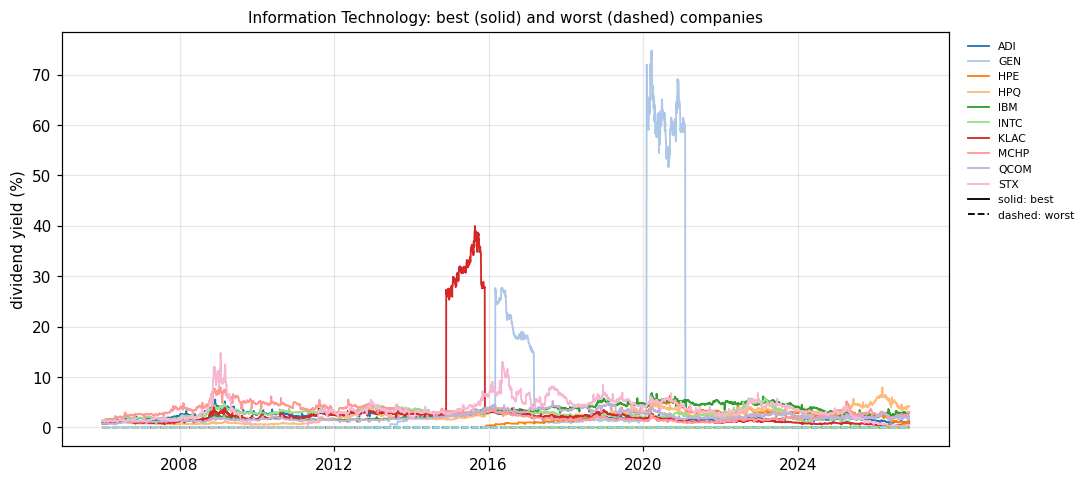
\includegraphics[width=1\textwidth]{appendix/dividend_yield/information_technology.png}
\caption{Information Technology: trailing dividend yield of the 10 companies with the highest (solid) and lowest (dashed) mean yield over the full history; percent.}
\end{figure}
\subsection{Materials}
\begin{figure}[H]
\centering
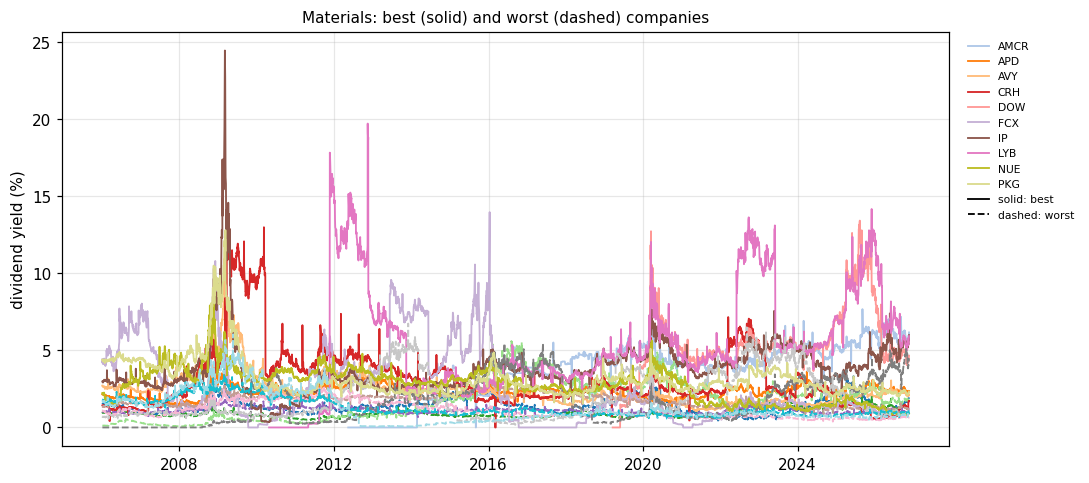
\includegraphics[width=1\textwidth]{appendix/dividend_yield/materials.png}
\caption{Materials: trailing dividend yield of the 10 companies with the highest (solid) and lowest (dashed) mean yield over the full history; percent.}
\end{figure}
\subsection{Utilities}
\begin{figure}[H]
\centering
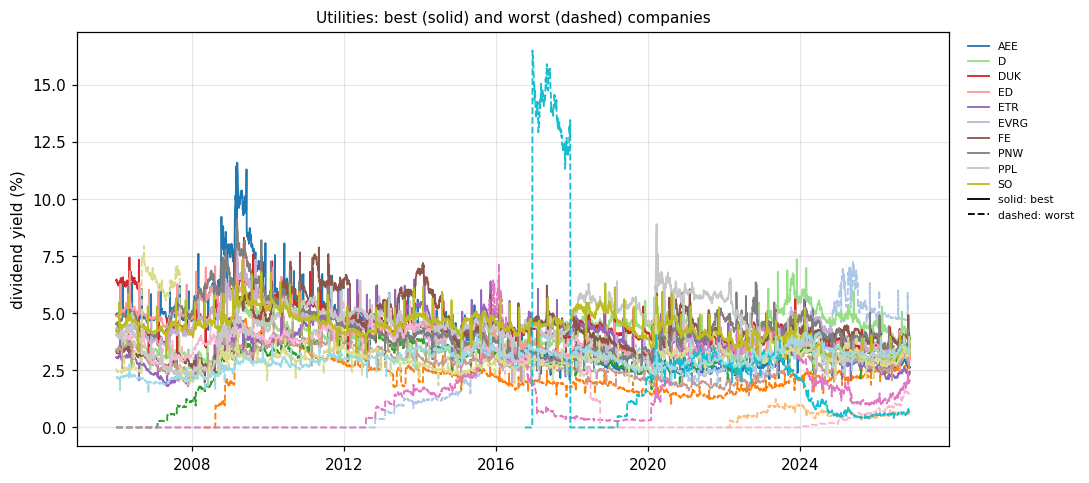
\includegraphics[width=1\textwidth]{appendix/dividend_yield/utilities.png}
\caption{Utilities: trailing dividend yield of the 10 companies with the highest (solid) and lowest (dashed) mean yield over the full history; percent.}
\end{figure}
\section{Data checks}
\label{app:data_checks}
Checks of the data behind the report: how many companies report each field per year, whether reported EPS agrees with net income divided by diluted shares, how long after the period end filings arrive (the point-in-time delay), whether every symbol has a full trading calendar (youngest first, which shows each company's age in the data), and the exchange rate for ZAR figures.

\begin{figure}[H]
\centering
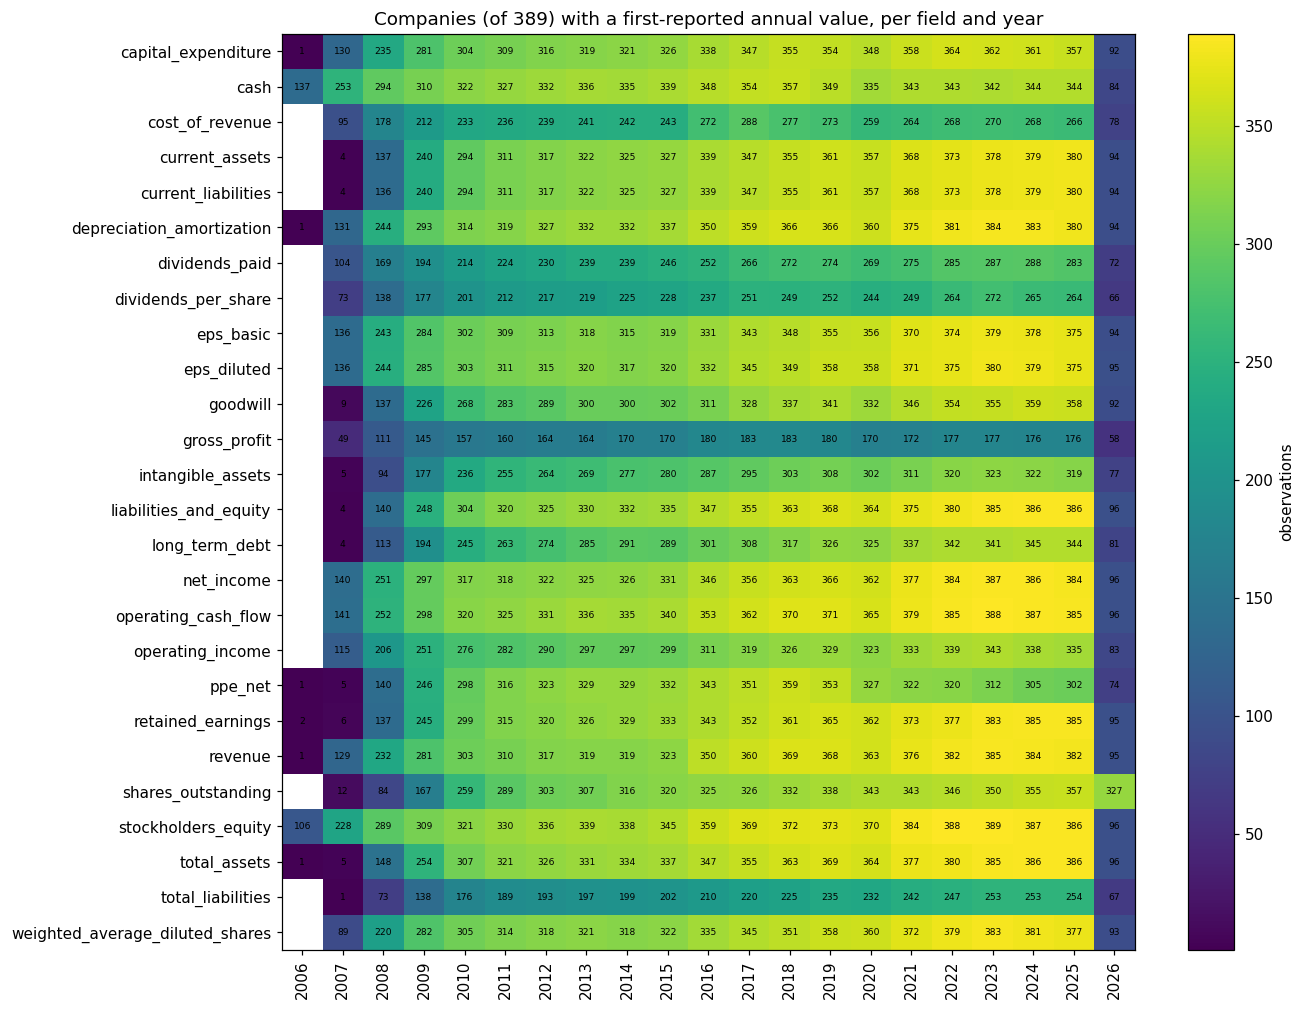
\includegraphics[width=1\textwidth]{appendix/data_checks/coverage.png}
\caption{Number of companies with a first-reported annual value, per field and fiscal year.}
\end{figure}
\begin{figure}[H]
\centering
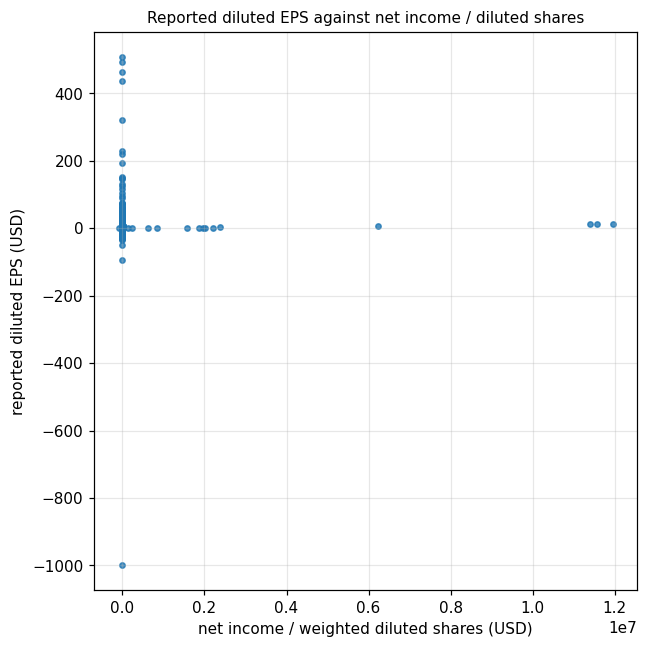
\includegraphics[width=1\textwidth]{appendix/data_checks/eps_check.png}
\caption{Reported diluted EPS against net income divided by weighted diluted shares, USD per share; points off the diagonal differ.}
\end{figure}
\begin{figure}[H]
\centering
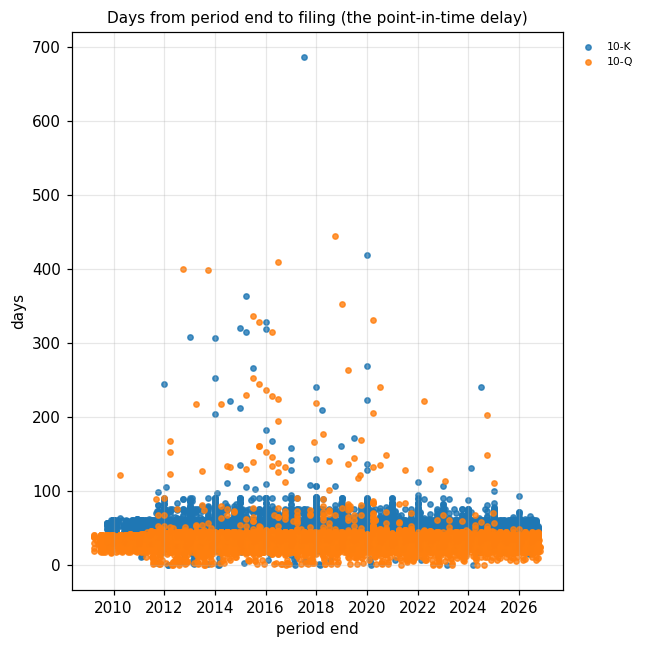
\includegraphics[width=1\textwidth]{appendix/data_checks/filing_lag.png}
\caption{Days from period end to filing for each 10-K and 10-Q.}
\end{figure}
\begin{figure}[H]
\centering
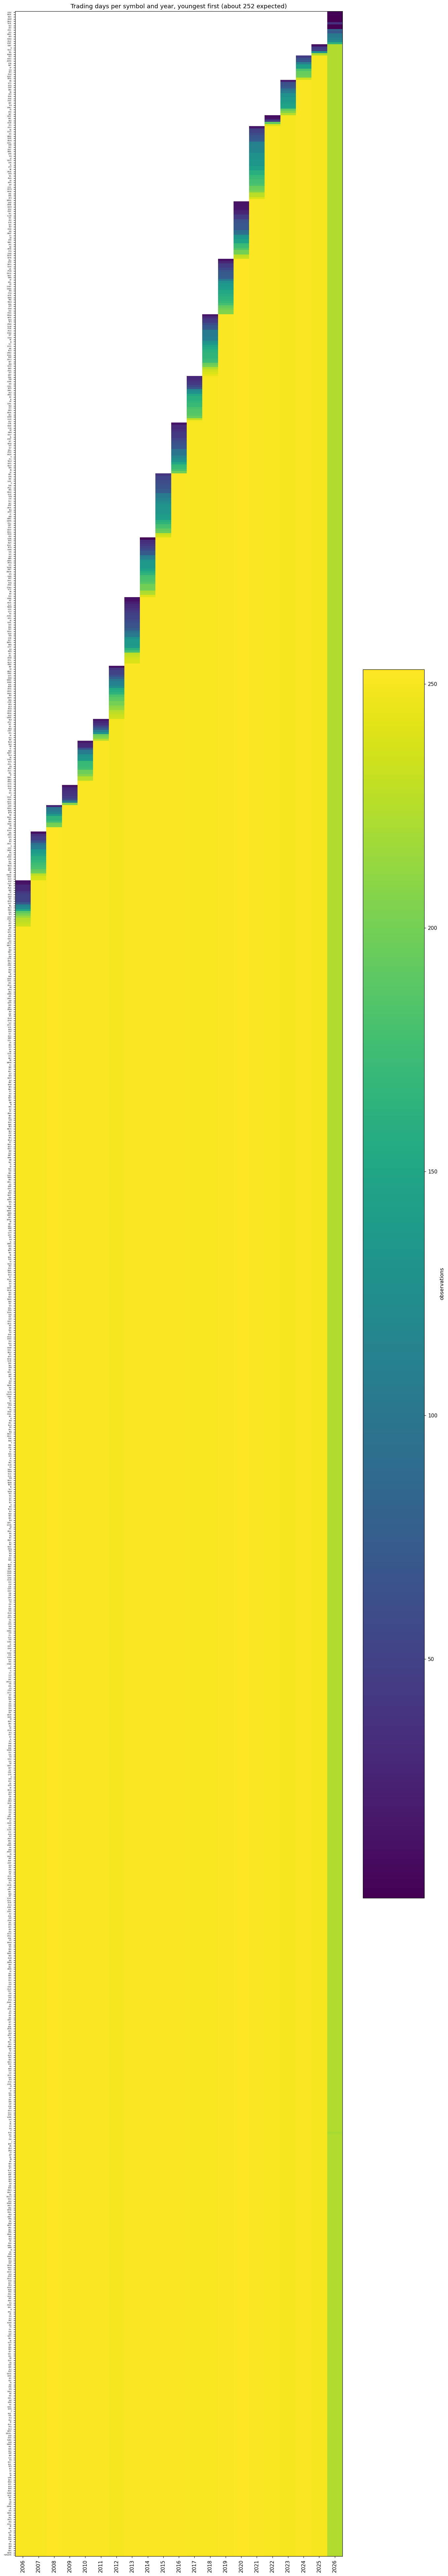
\includegraphics[width=1\textwidth]{appendix/data_checks/trading_days.png}
\caption{Trading days per symbol and year, youngest symbols at the top; a row starts in the year the symbol first traded.}
\end{figure}
\begin{figure}[H]
\centering
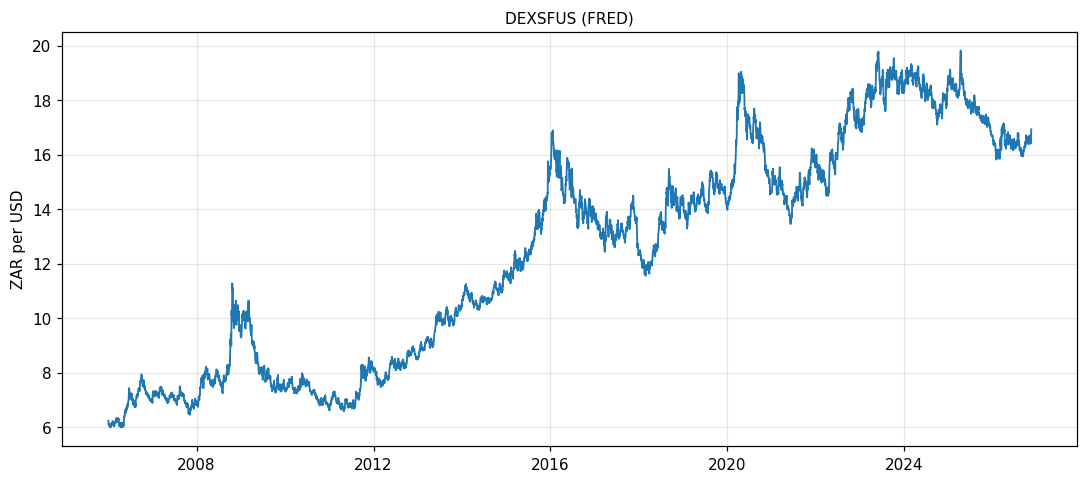
\includegraphics[width=1\textwidth]{appendix/data_checks/DEXSFUS.png}
\caption{USD/ZAR exchange rate (FRED DEXSFUS), rand per US dollar.}
\end{figure}
\begin{figure}[H]
\centering
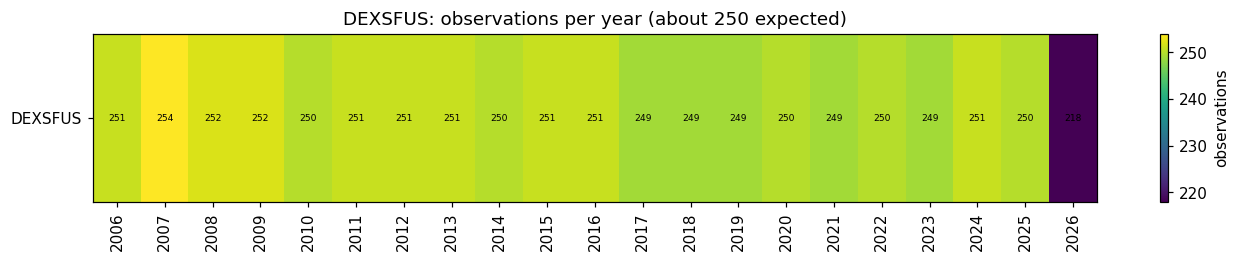
\includegraphics[width=1\textwidth]{appendix/data_checks/DEXSFUS_coverage.png}
\caption{Exchange-rate observations per year.}
\end{figure}
\end{document}
